\documentclass[a4paper,preprint,11pt]{article}
%%%\usepackage{setspace}
%\doublespacing
\usepackage{amsmath}
\usepackage{graphicx}
\usepackage{amsthm}
\usepackage{amssymb}
\usepackage{bm}
\usepackage{multicol}
\usepackage{wrapfig}
\usepackage{paralist} 
\usepackage{graphics} 
\usepackage{epsfig} 
\usepackage{ulem}
\usepackage{color}
\usepackage[margin=3cm]{geometry}
%%%\usepackage[pagewise]{lineno}\linenumbers
%\reversemarginpar
%\usepackage[colorinlistoftodos]{todonotes}
%\usepackage{epstopdf}% To incorporate .eps illustrations using PDFLaTeX, etc.
%\usepackage{subfigure}% Support for small, `sub' figures and tables
%\usepackage[colorinlistoftodos]{todonotes}
%\usepackage[utf8]{inputenc}
%\usepackage{epsfig}
%\usepackage{graphics}
%\usepackage{amsmath}
%\usepackage{amssymb}
%\usepackage{bm}
%\usepackage{ulem}
%\usepackage{geometry}
% \geometry{a4paper,
% total={170mm,257mm},
% left=20mm,
% top=20mm,}
% \usepackage{setspace}
%\doublespacing
\newtheorem{theorem}{Theorem}[section]
\newtheorem{corollary}[theorem]{Corollary}
\newtheorem{lemma}[theorem]{Lemma}
\newtheorem{proposition}[theorem]{Proposition}
\newtheorem{definition}[theorem]{Definition}
\newtheorem{example}[theorem]{Example}
\newtheorem{remark}[theorem]{Remark}
\newcommand{\AT}[1]{\textcolor{blue}{{#1}}}
\newcommand{\XAT}[1]{\xout{\textcolor{blue}{{#1}}}}
\title{Slow-passage through a Hopf-like bifurcation} 
%
\author{}
%

\newcommand\New[1]{\textcolor[rgb]{0.75,0,0.5}{{ #1}}}
\newcommand\Notes[1]{\textcolor[rgb]{0.2,0,0.8}{{ #1}}}
\newcommand\ToDo[1]{\textcolor[rgb]{1,0,0.2}{{ #1}}}



%%% spacing math mode
\usepackage[nodisplayskipstretch]{setspace}
\setstretch{1.25}


\begin{document}


\maketitle
\tableofcontents

\break

%\begin{abstract}
%\end{abstract}

\pagestyle{myheadings}
\thispagestyle{plain}




\section{Introduction}
Our aim is to find a minimal model to reproduce the slow passage effect. Firstly, we try using a 2 dimensional model to reproduce the slow passage through a Hopf bifurcation in the PWL context
\begin{align}
\dot{x} & =f(x)-y\\
\dot{y} & =x-a
\end{align}   
with 
\[
f(x)=\left\{
\begin{array}{ll}
-mx & x\leq 0,\\
kx & x \geq 0
\end{array}
\right.
\]
This system exhibits an unique equilibrium at $(a,f(a))$ and the Jacobian matrix at the equibrium is 
\[
 \begin{pmatrix}
  f'(a) & -1\\
  1	& 0
 \end{pmatrix}.
\]
Then, the equilibrium point changes its stability at $a=0$ passing from being stable at $a<0$ to being unstable at $a>0$. Assuming $0<k<m<2$, then the system exhibits a supercritical Hopf bifurcation at $a=0$.

We now consider a slow drift on the parameter $a(t)=a_0+\varepsilon t$ to force a slow passage through the Hopf.  

Following we present some simulations showing the effect of the slow passage in the PWL setting, see Figure 1 and Figure 2. 

\begin{figure}[h!]
  \begin{center}
  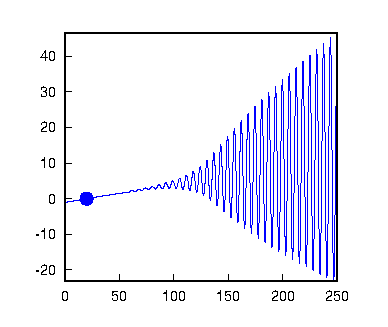
\includegraphics[width=9cm]{Sp_PWL_dibu1.eps}
  \end{center}
  \caption{Coordinate $x(t)$ versus $t$ for parameters $m=0.2,k=0.1,a_0=-1,\varepsilon=0.05$. The point corresponds with the Hopf. It can be observed the delay in the amplitude due to the passage through the Hopf.}
\end{figure}

\begin{figure}[h!]
  \begin{tabular}{cc}
    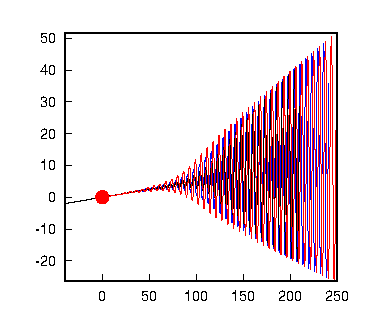
\includegraphics[width=6.5cm]{Sp_PWL_dibu2.eps} 
    &
    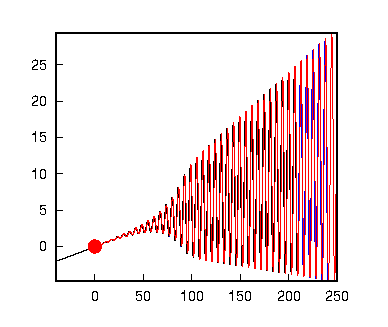
\includegraphics[width=6.5cm]{Sp_PWL_dibu3.eps}
  \end{tabular}
  \caption{Coordinate $x(t)$ versus $t$ for parameters $k=0.1,\varepsilon=0.05$ and different values of $m$ and $a_0$. (a) For $m=0.2$, blue curve corresponds to $a_0=-1$, black curve to $a_0=-0.2$ and red curve to $a_0=0$. The delay in the amplitude seems not to be dependent on the the nevative parameter $a_0$ is. (b) For $m=1$, black curve corresponds to $a_0=-2$, blue curve to $a_0=-0.45$ and red curve to $a_0=0$. In this case, the delay in the amplitude due to the passage through the Hopf is the same for the three solutions It is probably due to the increase in the contraction as we have increased parameter $m$, which force that three solutions seems the same as they arrive at the Hopf point. Moreover, the delay is smaller than the delay in the previous examples, note that solutions achieve the expected amplitude at time 100 approx.}
\end{figure}


% \begin{figure}[h!]
%   \begin{center}
%   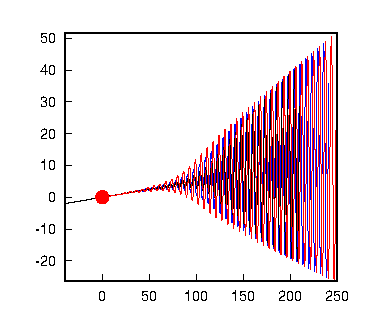
\includegraphics[width=9cm]{Sp_PWL_dibu2.eps}
%   \end{center}
%   \caption{Coordinate $x(t)$ versus $t$ for parameters $m=0.2,k=0.1,\varepsilon=0.05$ and different values of $a_0$. Thus, blue curve corresponds to $a_0=-1$, black curve to $a_0=-0.2$ and red curve to $a_0=0$. It can be observed that the delay in the amplitude due to the passage through the Hopf is bigger as the value of $a_0$ is more negative.}
% \end{figure}
% 
% 
% \begin{figure}[h!]
%   \begin{center}
%   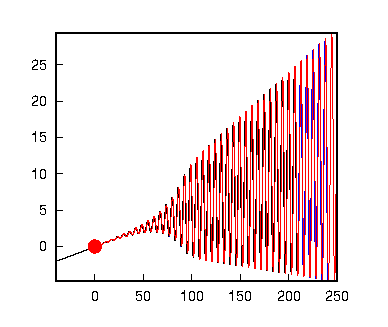
\includegraphics[width=8cm]{Sp_PWL_dibu3.eps}
%   \end{center}
%   \caption{Coordinate $x(t)$ versus $t$ for parameters $m=1,k=0.1,\varepsilon=0.05$ and different values of $a_0$. Thus, black curve corresponds to $a_0=-2$, blue curve to $a_0=-0.45$ and red curve to $a_0=0$. In this case, the delay in the amplitude due to the passage through the Hopf is the same for the three solutions It is probably due to the increase in the contraction as we have increased parameter $m$, which force that three solutions seems the same as they arrive at the Hopf point. Moreover, the delay is smaller than the delay in the previous examples, note that solutions achieve the expected amplitude at time 100 approx.}

\begin{figure}[ht]
  \begin{center}
  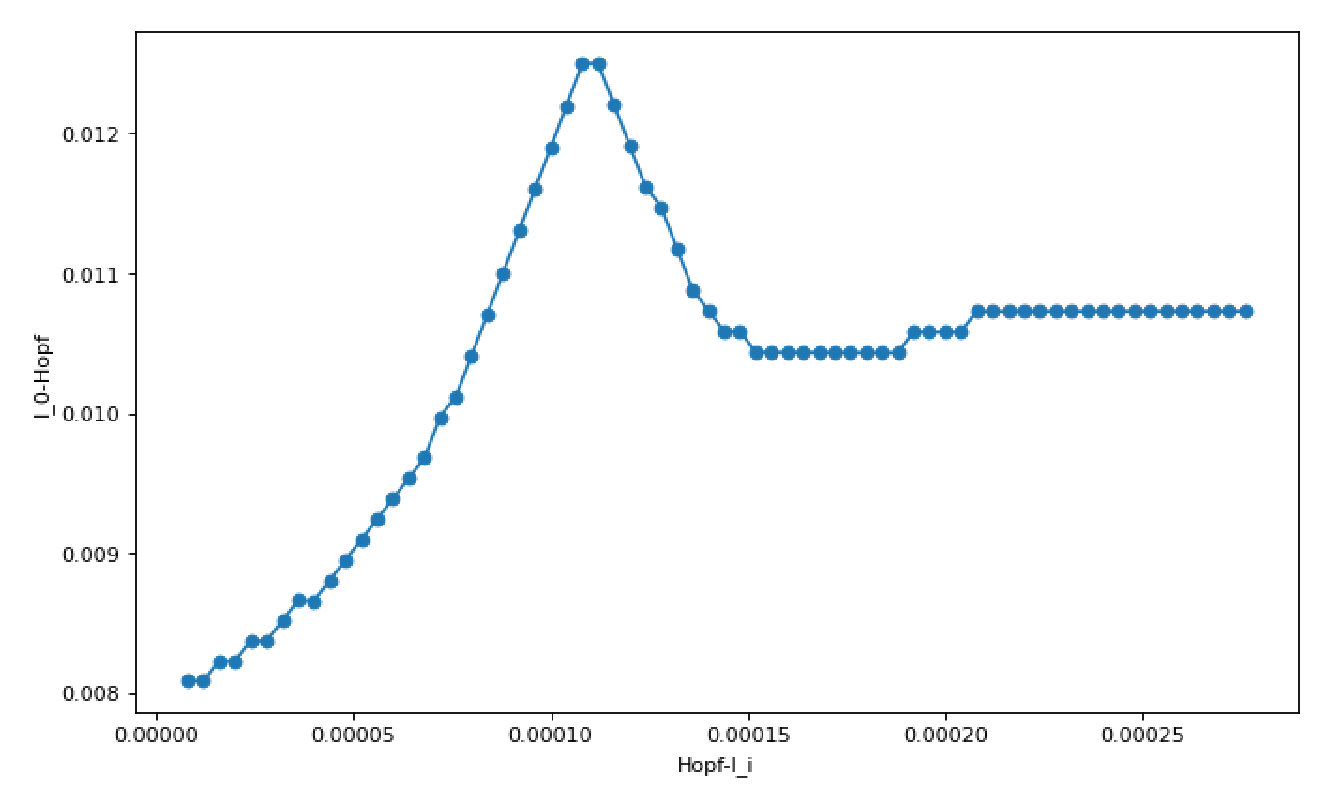
\includegraphics[width=8cm]{Sp_PWL_dibu4.eps}
  \end{center}
  \caption{Representation of the delay versus the $a_0$ parameter in the PWL version of the Morris-Lecar model. It can be seen that after a maximun in the delay, the delay saturates and remains constant. This fact could be explained from Figure 3.   
}
\end{figure}

\begin{remark} It could be concluded that the slow passage through the Hopf-like in the PWL context does not behave in the same way that it does through the classical Hopf bifurcation. We note that the contraction effect of the slow manifold depends on the real part of the eigenvalues of the Jacobian matrix. Hence, the smaller is the real part of the eigenvalues, the smaller is the contraction effect, and the solutions for different values of $a_0$ remains different at the Hopf point. Thus the delay is different for different values of $a_0$. On the contrary the bigger is the real part of the eigenvalues, the  bigger is the contraction, and thus solutions for different values of $a_0$ seems to be equal at the Hopf point. Therefore, the delay is the same for every  $a_0$. 

In the smooth context the eigenvalues varies when the parameter does, which implies that close to the fold its real part is small, which implies the existence of different delays for different values of $a_0$. On the contrary, in the PWL context, the eigenvalues do not change with the parameter, so when $m$ is big enough the contraction makes all solutions to seem the same at the Hopf point, so that the delay is the same for every $a_0$.
\end{remark}



\section{Study of 2-regions model}

\subsection{Analytical approach}

The local expression of the flow is

\begin{align*}
x_L(t)&=a(t)-m\varepsilon+
  e^{-\frac {m}{2}t} \left(
      C_1 \cos\left(\frac {\sqrt{4-m^2}}2t \right)+
      C_2 \sin\left(\frac {\sqrt{4-m^2}}2t \right)
    \right),\\
y_L(t)&=-m(a(t)-m\varepsilon)-\varepsilon\\
  &+e^{-\frac {m}{2}t} \left(
      -\frac{C_2\sqrt{4-m^2}+C_1m}2 \cos\left(\frac {\sqrt{4-m^2}}2t \right)
      +\frac{C_1\sqrt{4-m^2}-C_2 m}2 \sin\left(\frac {\sqrt{4-m^2}}2t \right)
    \right),
\end{align*}
on the left region, and 
\begin{align*}
x_R(t)&=a(t)+k\varepsilon+
  e^{\frac {k}{2}t} \left(
      D_1 \cos\left(\frac {\sqrt{4-k^2}}2t \right)+
      D_2 \sin\left(\frac {\sqrt{4-k^2}}2t \right)
    \right),\\
y_R(t)&=k(a(t)+k\varepsilon)-\varepsilon\\
  &+e^{\frac {k}{2}t} \left(
      \frac{kD_1-D_2\sqrt{4-k^2}}2 \cos\left(\frac {\sqrt{4-k^2}}2t \right)
      +\frac{kD_2+D_1\sqrt{4-k^2}}2 \sin\left(\frac {\sqrt{4-k^2}}2t \right)
    \right)
\end{align*}
on the right region. It can be written respect to the initial conditions $x_0,y_0,a_0$ as:

\begin{align*}
x_R(t)&=a(t)+k\varepsilon+
  e^{\frac {k}{2}t} \left(
      (x_0-a_0-k\epsilon) \cos\left(\frac {\sqrt{4-k^2}}2t \right)+\right. \\
      & \left. \frac{k(a_0+k\epsilon+x_0)-2(y_0+\epsilon)}{\sqrt{4-k^2}} \sin\left(\frac {\sqrt{4-k^2}}2t \right)
    \right),\\
y_R(t)&=k(a(t)+k\varepsilon)-\varepsilon\\
  &+e^{\frac {k}{2}t} \left(
      (-k(a_0+k\epsilon)+(y_0+\epsilon))\cos\left(\frac {\sqrt{4-k^2}}2t \right) \right. \\
      & \left. +\frac{k^2(a_0+k\epsilon)-k(y_0+\epsilon)+2(x_0-a_0-k\epsilon)}{\sqrt{4-k^2}} \sin\left(\frac {\sqrt{4-k^2}}2t \right)
    \right)
\end{align*}


\subsection{Some graphical behaviors}

\begin{table}[ht]
 %   \centering
    \begin{tabular}{ccc}
	$\epsilon=0.05$ & $\epsilon=0.01$ & $\epsilon=0.005$  \\
    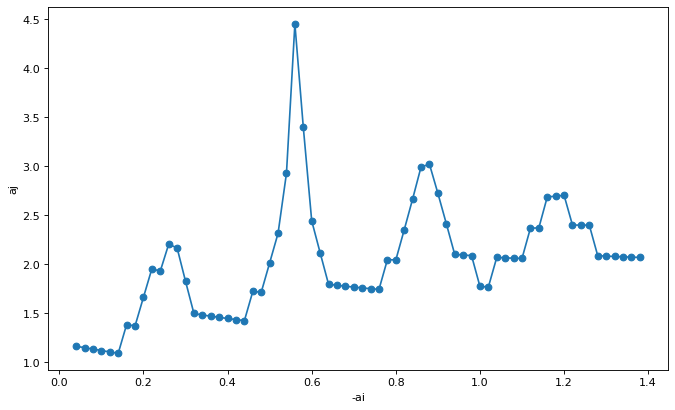
\includegraphics[scale=0.2]{m02e005.png} & 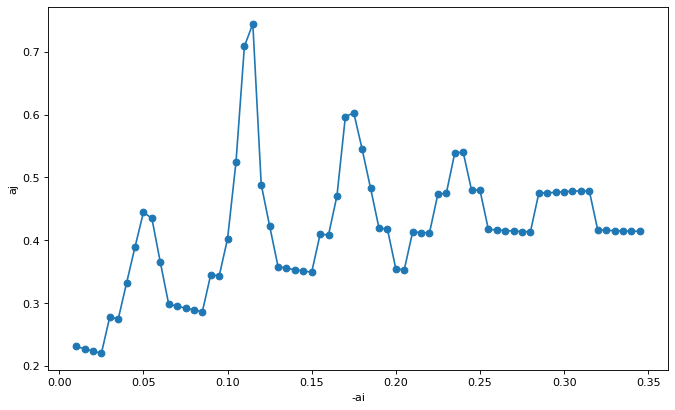
\includegraphics[scale=0.2]{m02e001.png} & 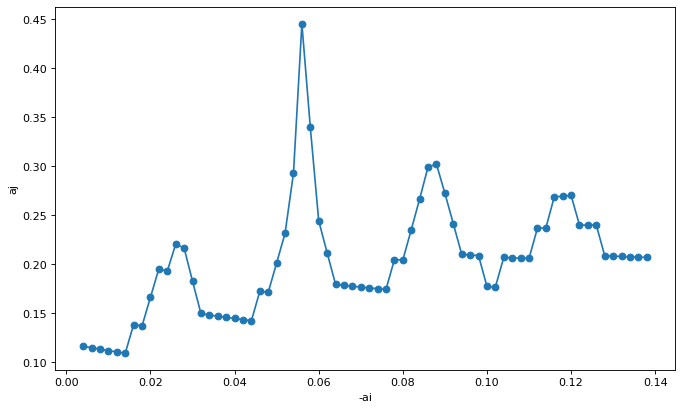
\includegraphics[scale=0.2]{m02e0005.png}  \\
                        & $m=0.2$   &  \\
    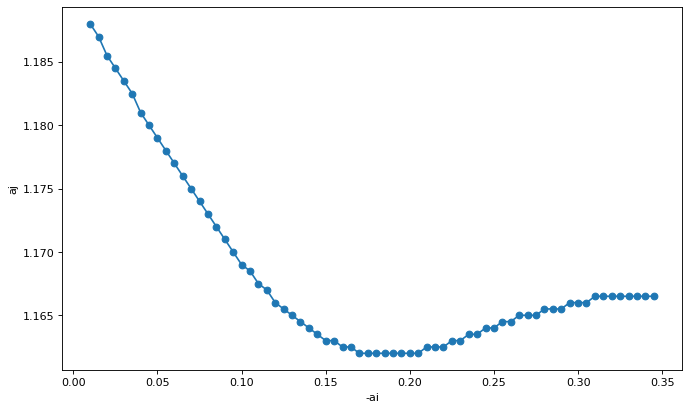
\includegraphics[scale=0.2]{m1e005.png} & 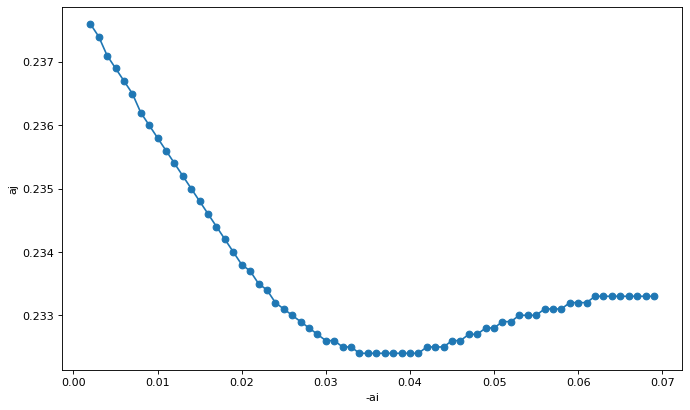
\includegraphics[scale=0.2]{m1e001.png} & 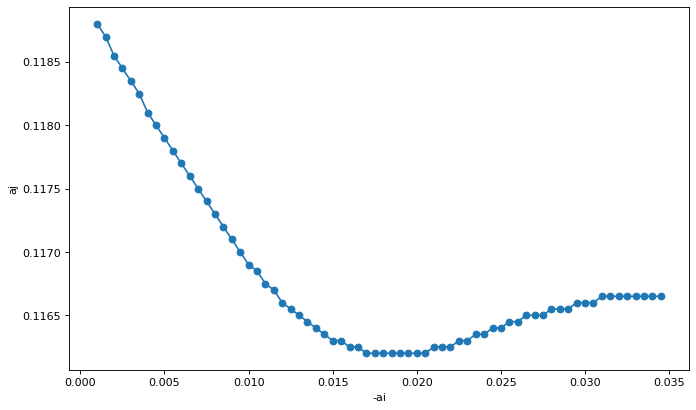
\includegraphics[scale=0.2]{m1e0005.png}  \\
			& $m=1$   &  \\
    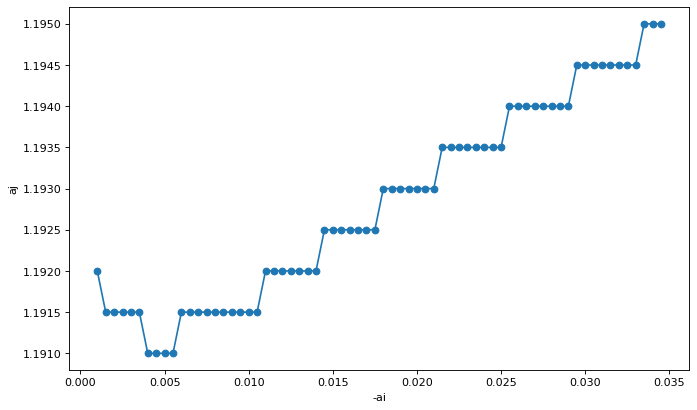
\includegraphics[scale=0.2]{m175e005.png} & 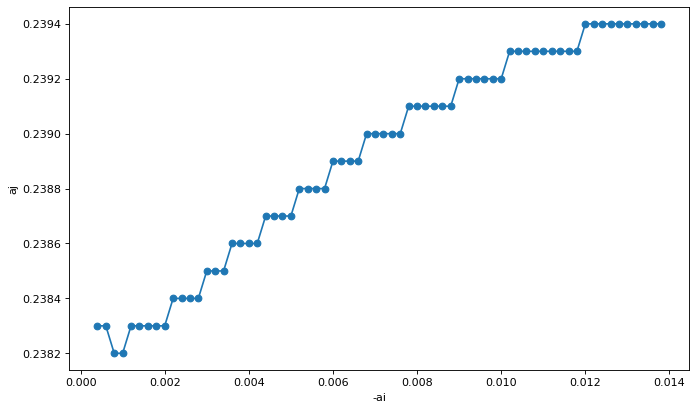
\includegraphics[scale=0.2]{m175e001.png} & 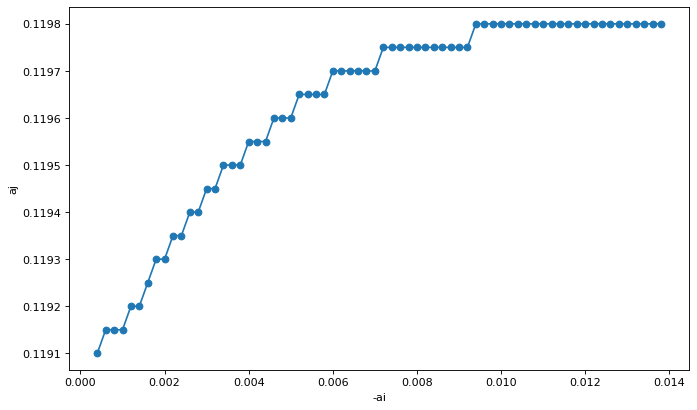
\includegraphics[scale=0.2]{m175e0005.png}  \\
			& $m=1.75$   &  \\
    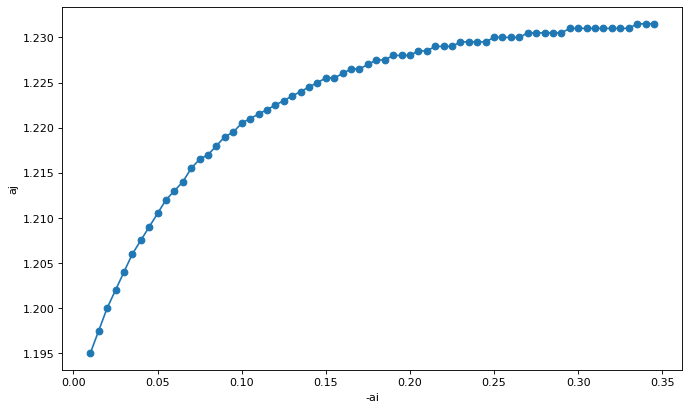
\includegraphics[scale=0.2]{m25e005.png} & 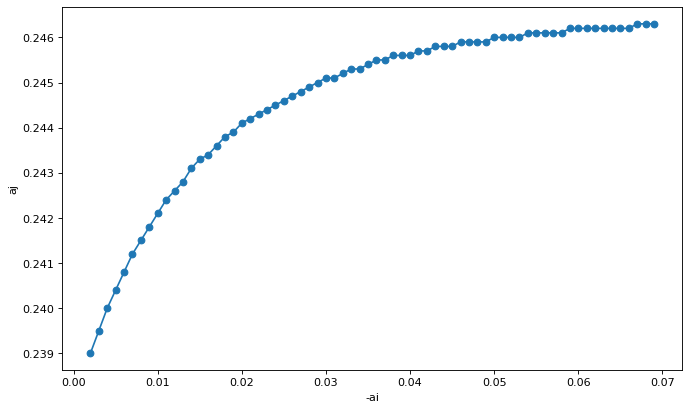
\includegraphics[scale=0.2]{m25e001.png} & 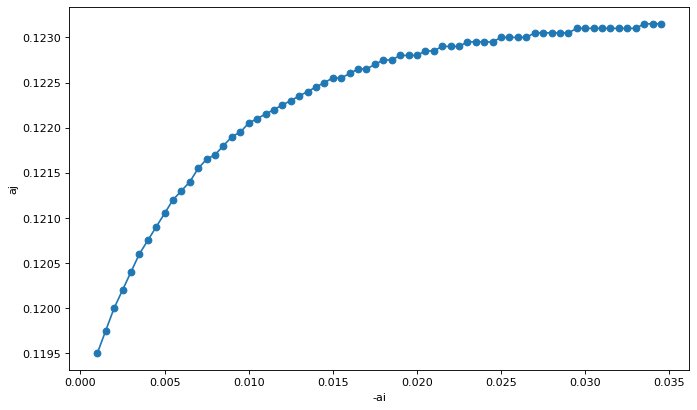
\includegraphics[scale=0.2]{m25e0005.png}  \\
			& $m=2.5$   &  
    \end{tabular}
    \caption{\textbf{Slow passage through a PWL Hopf for $k=0.1$ and different values of $m$ and $\epsilon$}. From these simulations it can be concluded that parameter $m$, that is, the divergence of the system, is related with the shape of the graph of the function input-output. Moreover, the parameter $\varepsilon$, that is the velocity of the passage, is related with the size of the delay but also with a translation of the graph. Both efect seem to be  $O(\varepsilon)$.
    }
    \label{tab:plots}
\end{table}


\subsection{Ellipse calculation}
Let us consider the plane $x_0=0$. Then,
\begin{enumerate}
    \item Taking the initial conditions $x_0=0$, $y_0=-\epsilon$ and $a_0=-k\epsilon$, we have that
\begin{align*}
x^*_R(t)&=\epsilon t,\\
y^*_R(t)&=\epsilon kt-\epsilon\\
a^*_R(t)&=\epsilon t-k\epsilon
\end{align*}
which is the invariant manifold in the right-side of the system and it is a straight line.
\item On the other hand, by considering only the plane  $x_0=0$, we have
\begin{align*}
x_R(t)&=\epsilon t + a_0 +k\varepsilon+
  e^{\frac {k}{2}t} \left(
      (-a_0-k\epsilon) \cos\left(\frac {\sqrt{4-k^2}}2t \right)+\right. \\
      & \left. \frac{k(a_0+k\epsilon)-2(y_0+\epsilon)}{\sqrt{4-k^2}} \sin\left(\frac {\sqrt{4-k^2}}2t \right)
    \right),\\
y_R(t)&=k(\epsilon t + a_0 +k\varepsilon)-\varepsilon\\
  &+e^{\frac {k}{2}t} \left(
      (-k(a_0+k\epsilon)+(y_0+\epsilon))\cos\left(\frac {\sqrt{4-k^2}}2t \right) \right. \\
      &  \left. +\frac{k^2(a_0+k\epsilon)-k(y_0+\epsilon)-2(a_0+k\epsilon)}{\sqrt{4-k^2}} \sin\left(\frac {\sqrt{4-k^2}}2t \right)
    \right)
a_R(t)=\epsilon t + a_0
\end{align*}
\item Then, $y_R(t)$ and $a(t)$ can be written in terms of $x_R(t)$ as
\begin{align*}
y_R(t)&=k x_R(t) - \epsilon +\\
  &+e^{\frac {k}{2}t} \left(
      (y_0+\epsilon)\cos\left(\frac {\sqrt{4-k^2}}2t \right) \right. \\
      &  \left. +\left( \frac{2(-a_0-k\epsilon)+k(y_0+\epsilon)}{\sqrt{4-k^2}} \right) \sin\left(\frac {\sqrt{4-k^2}}2t \right)
    \right)\\
a_R(t)&=x_R(t)-k\varepsilon-
  e^{\frac {k}{2}t} \left(
      (-a_0-k\epsilon) \cos\left(\frac {\sqrt{4-k^2}}2t \right)+\right. \\
      & \left. \frac{k(a_0+k\epsilon)-2(y_0+\epsilon)}{\sqrt{4-k^2}} \sin\left(\frac {\sqrt{4-k^2}}2t \right)
    \right),
\end{align*}
\item Then, $x_R(t),\ y_R(t)$ and $a(t)$ can be written as
\begin{align*}
x_R(t)&=a(t)+k\varepsilon-
  e^{\frac {k}{2}t} \left(
      (-a_0-k\epsilon) \cos\left(\frac {\sqrt{4-k^2}}2t \right)+\right. \\
      & \left. \frac{k(a_0+k\epsilon)-2(y_0+\epsilon)}{\sqrt{4-k^2}} \sin\left(\frac {\sqrt{4-k^2}}2t \right)
    \right),\\
y_R(t)&=k x_R(t) - \epsilon +\\
  &+e^{\frac {k}{2}t} \left(
      -(y_0+\epsilon)\cos\left(\frac {\sqrt{4-k^2}}2t \right) \right. \\
      &  \left. +\left( \frac{2(-a_0-k\epsilon) +k(y_0+\epsilon)}{\sqrt{4-k^2}} \right) \sin\left(\frac {\sqrt{4-k^2}}2t \right)
    \right),\\
a_R(t)&=\epsilon t + a_0
\end{align*}
\end{enumerate}

\textbf{Summarizing the previous notes we have that:} Given an initial condition on $x_0=0$, we have
\begin{align*}
    y_R(t)&=kx_R(t)-\epsilon+e^{\frac k 2 t} A_1\cos(\theta_1-\beta t)\\
    a_R(t) &=x_R(t)-k\epsilon+e^{\frac k 2 t} A_2\cos(\theta_2-\beta t)
\end{align*}

Then, we can compute the distance between the solution and the line such that
\begin{equation}\label{eq.x0}
\begin{pmatrix} x_R \\ y_R \\ a_R \end{pmatrix} =
\begin{pmatrix} 0 \\ -\epsilon \\ -k\epsilon \end{pmatrix} +
 x_R \begin{pmatrix} 1 \\ k \\ 1 \end{pmatrix} +e^{\frac k 2 t}
 \begin{pmatrix} 0 \\ A_1 \cos(\theta_1-\beta t) \\ A_2 \cos(\theta_2-\beta t)\end{pmatrix}
\end{equation}
This equation consists on a point plus a vector multiplied by $x_R$ and then an exponential term which depends on $t$. Then, we have a point on a straight line plus an oscillation. Then, the exponential term is related to the escape distance. We want to find $A_1$ and $A_2$. Since
$$
a\cos(\theta)+b\sin(\theta)=c\cos(\theta'),\quad\text{where }c^2=a^2+b^2,
$$
We will calculate $c^2$ in each $y_R$ and $a$ case.
$$
y_R-kx_R+\epsilon = \underbrace{(y_0+\epsilon)}_{a_1}\cos + \underbrace{\frac{1}{\sqrt{4-k^2}}(k(y_0+\epsilon)-2(a_0+k\epsilon))}_{b_1}\sin.
$$
we calculate $a_1^2+b_1^2$:
$$
a_1^2+b_1^2 = \frac{4}{4-k^2}((y_0+\epsilon)^2+(a_0+k\epsilon)(a_0-ky_0))
$$
The $a$ case is similar:
$$
a-x_R+k\epsilon = -\underbrace{(-a_0-k\epsilon)}_{a_2}\cos - \underbrace{\frac{k(a_0+k\epsilon)-2(y_0+\epsilon)}{\sqrt{4-k^2}}}_{b_2}\sin. 
$$
the same expression appears as in the previous case. Thus
$$
\boxed{A_i^2 = \frac{4}{4-k^2}((y_0+\epsilon)^2+(a_0+k\epsilon)(a_0-ky_0))}
$$


%%\subsection{Plot the spirals of all the points that lasts t* to escape}
\subsection{Analytical expression of the ellipse}
Since the expression of the $A_i$ is $A_i^2 = \frac{4}{4-k^2}((y_0+\epsilon)^2+(a_0+k\epsilon)(a_0-ky_0))$, we know that the escape expression from $x_R$ is
$$
e^{\frac{k}{2}t}A_i = \delta.
$$
$\delta>0$ is the threshold that we put, and $t$ is the time to pass this threshold. We can square all sides of the equality, since they are positives. Therefore,
$$
e^{kt}A_i^2 = \delta^2 \Longrightarrow (y_0+\epsilon)^2+(a_0+k\epsilon)(a_0-ky_0) - \frac{4-k^2}{4}e^{-kt}\delta = 0.
$$
Since the ellipse is centered in $y_0=-\epsilon$, $z_0=-k\epsilon$, we realize the change $y_0=-\epsilon+y$, $z_0=-k\epsilon+z$. As a result, the previous expression changes to the simpler expression
$$
y^2-kzy+z^2 - \frac{4-k^2}{4}e^{-kt}\delta = 0.
$$
This is a second degree polynomial in terms of $y$. The solutions are
$$
y = \frac{kz\pm\sqrt{(k^2-4)(z^2-e^{-kt}\delta^2)}}{2}.
$$
This is the explicit expression of the ellipses. It gives us the form of the pair of points that satisfy the ellipse.
$$
(\frac{kz\pm\sqrt{(k^2-4)(z^2-e^{-kt}\delta^2)}}{2},z).
$$
These points are defined in $z\in[-e^{-\frac{k}{2}t}\delta,e^{-\frac{k}{2}t}\delta]$.

%%\textbf{2. which initial conditions require a time $t\geq t^*$ to escape?} We note that, the `radius' of the ellipse is
\subsection{Time Scaping}
We recall that the `radius' of the ellipse is
$$
y^2-kzy+z^2 = \frac{4-k^2}{4}e^{-kt}\delta \rightarrow f(t)=\frac{4-k^2}{4}e^{-kt}.
$$
Then, we must study this radius. $f'(t)=-k\frac{4-k^2}{4}e^{-kt}<0$ is a decreasing function. Thus, we must take a lower $t$ to find a bigger radius.
Hence, given $t^*$, for all $t>t^*$, we have
$$
\frac{4-k^2}{4}e^{-kt^*}\delta > \frac{4-k^2}{4}e^{-kt}\delta.
$$ 
All points of the ellipse $f(t)$ are inner points of the ellipse of $f(t^*)$. However, this shows us the time-scape depending the time $t$. If we want to check through the variables, we must use another technique. We recall that
\begin{equation}\label{eq.x01}
\begin{pmatrix} x_R \\ y_R \\ a_R \end{pmatrix} =
\begin{pmatrix} 0 \\ -\epsilon \\ -k\epsilon \end{pmatrix} +
 x_R \begin{pmatrix} 1 \\ k \\ 1 \end{pmatrix} +e^{\frac k 2 t}
 \begin{pmatrix} 0 \\ A_1 \cos(\theta_1-\beta t) \\ A_2 \cos(\theta_2-\beta t)\end{pmatrix}
\end{equation}
is the solution of our system on the right side. Using the 2nd and 3rd equations, we deduce
$$
y_R-y_0 = Ae^{\frac{k}{2}t}\cos(\theta_1+\xi_k t)
a_R-a_0 = Ae^{\frac{k}{2}t}\cos(\theta_2+\xi_k t)
$$
$\xi_k=\frac{\sqrt{4-k^2}}{2}$ and $\theta_1$, $\theta_2$ do not depend on time. In fact,
$$
\tan\theta_1 = \frac{-k(y_0+\epsilon)+2(a_0+k\epsilon)}{\sqrt{4-k^2}(y_0+\epsilon)}
$$
$$
\tan\theta_2 = \frac{k(a_0+k\epsilon)-2(y_0+\epsilon)}{\sqrt{4-k^2}(a_0+k\epsilon)}
$$
Moreover,
$$
\begin{array}{ccl}
(y_R-y_0)+(z_R-z_0) & = & Ae^{\frac{k}{2}t}\Big(\cos(\theta_1+\xi_k t) + \cos(\theta_2+\xi_k t)\Big) \\
& = & Ae^{\frac{k}{2}t}\Big(\sin(\theta_1+\xi_k t+\frac{\pi}{2}) + \sin(\theta_2+\xi_k t+\frac{\pi}{2})\Big) \\
& = & 2Ae^{\frac{k}{2}t}\sqrt{1+\cos(\theta_1-\theta_2)}\sin(\xi_kt+\frac{\pi}{2} + \varphi)
\end{array}
$$
where
$$
\tan\varphi = \frac{\sin\theta_1+\sin\theta_2}{\cos\theta_1+\cos\theta_2}
$$
This difference can be null and therefore, we must consider the `norm':
$$
\begin{array}{ccl}
(y_R-y_0)^2+(z_R-z_0)^2 & = & A^2e^{kt}\Big(\cos^2(\theta_1+\xi_k t) + \cos^2(\theta_2+\xi_k t)\Big) \\
& = & A^2e^{kt}\left[1 + \frac{1}{2}\left(\cos(2(\theta_1+\xi_kt)) + \cos(2(\theta_2+\xi_kt)) \right)\right] \\
& = & A^2e^{kt}\left[1 + \frac{1}{2}\left(\sin(2\theta_1+2\xi_kt+\frac{\pi}{2})) + \sin(2\theta_1+2\xi_kt+\frac{\pi}{2})) \right)\right] \\
& = & A^2e^{kt}\left[1 + \frac{1}{2}\left(c\sin(2\xi_kt+\frac{\pi}{2}+\varphi) \right)\right]
\end{array}
$$
In this case, $c=\sqrt{2(1+\cos(2(\theta_1-\theta_2)))}= k$. Therefore, it does not nullify the previous expression:
$$
(y_R-y_0)^2+(z_R-z_0)^2 > 0.
$$
However, this should be improvable, because the term $\sin(2\xi_kt+\frac{\pi}{2}+\varphi)$ makes some undesired fluctuations. Improving this could require some trigonometric combination, or maybe it cannot be improved.

\subsection{Graphic computation}
In the following images, we can see the result for different thresholds. In these cases, $m=1$ and $\epsilon=0.25$.

%%% The minor and major axis of the ellipse are with a slope of $1$ and $-1$.

\begin{center}
\begin{tabular}{cc}
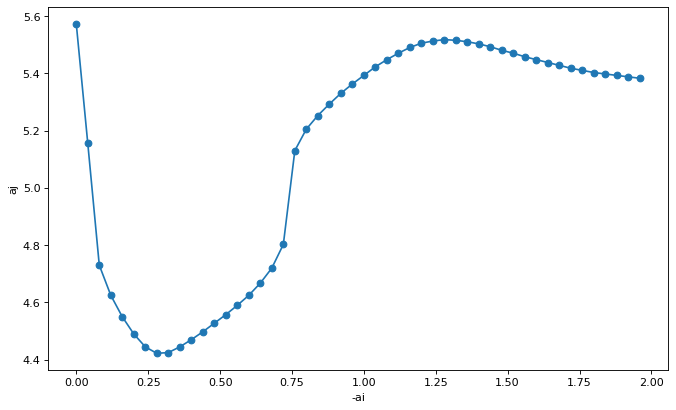
\includegraphics[scale=0.35]{Corba_y-y0_z-z0_0_6.png} &
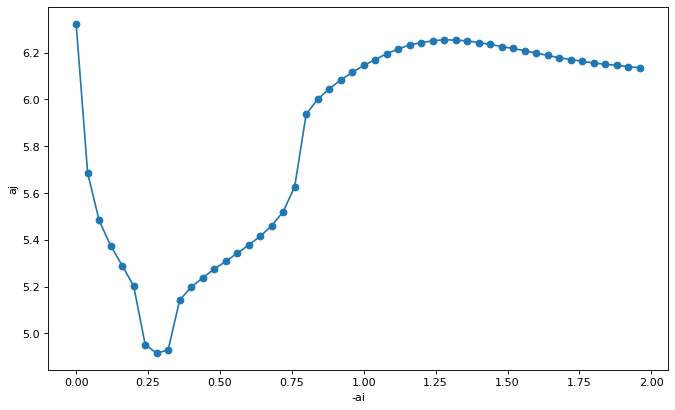
\includegraphics[scale=0.35]{Corba_y-y0_z-z0_0_8.png} \\
thres $=0.6$ & thres $=0.8$ \\
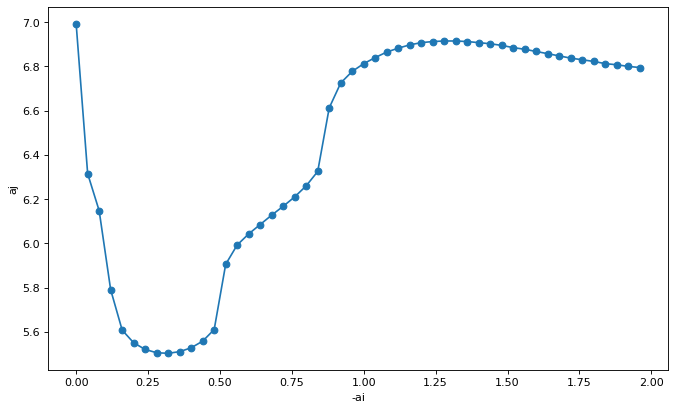
\includegraphics[scale=0.35]{Corba_y-y0_z-z0_1.png} &
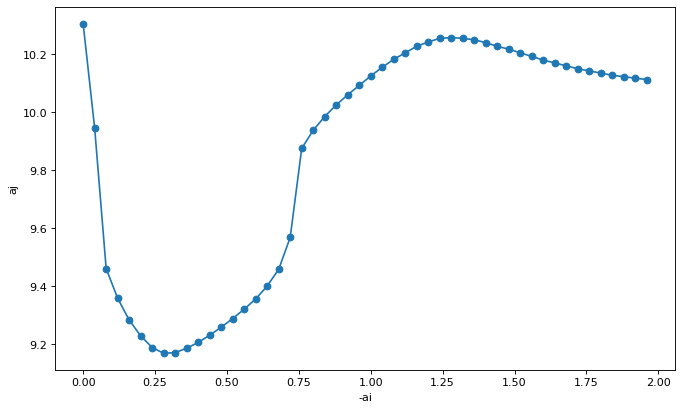
\includegraphics[scale=0.35]{Corba_y-y0_z-z0_4.png} \\
thres $=1$ & thres $=4$ \\
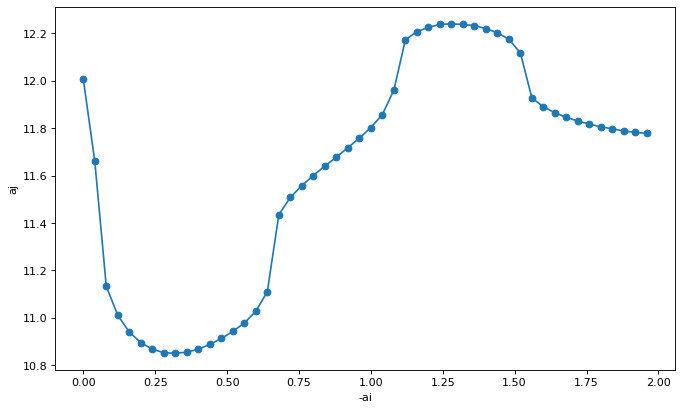
\includegraphics[scale=0.35]{Corba_y-y0_z-z0_8.png} &
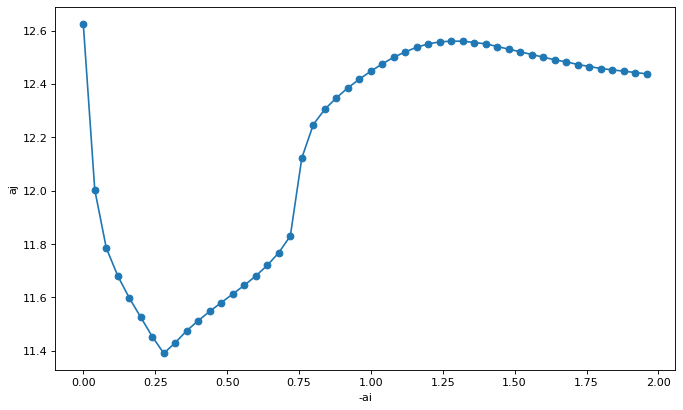
\includegraphics[scale=0.35]{Corba_y-y0_z-z0_10.png} \\
thres $=8$ & thres $=10$
%\caption{$m=1$, $\epsilon=0.25$.}
\end{tabular}
\end{center}
We try to match results with the spiral. $thres=0.6$ seems good enough:
\begin{center}
\begin{tabular}{cc}
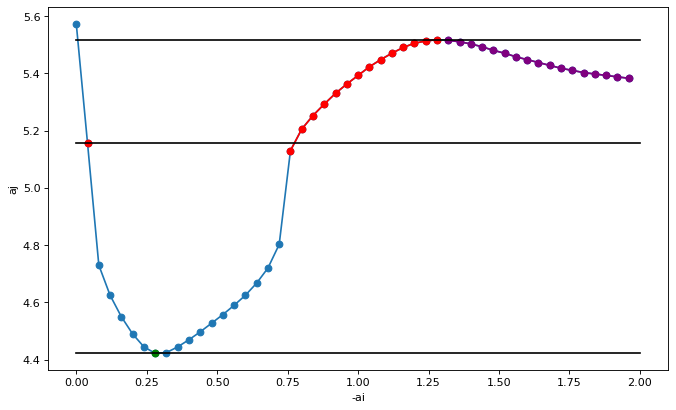
\includegraphics[scale=0.35]{CorbaMarcada.png} &
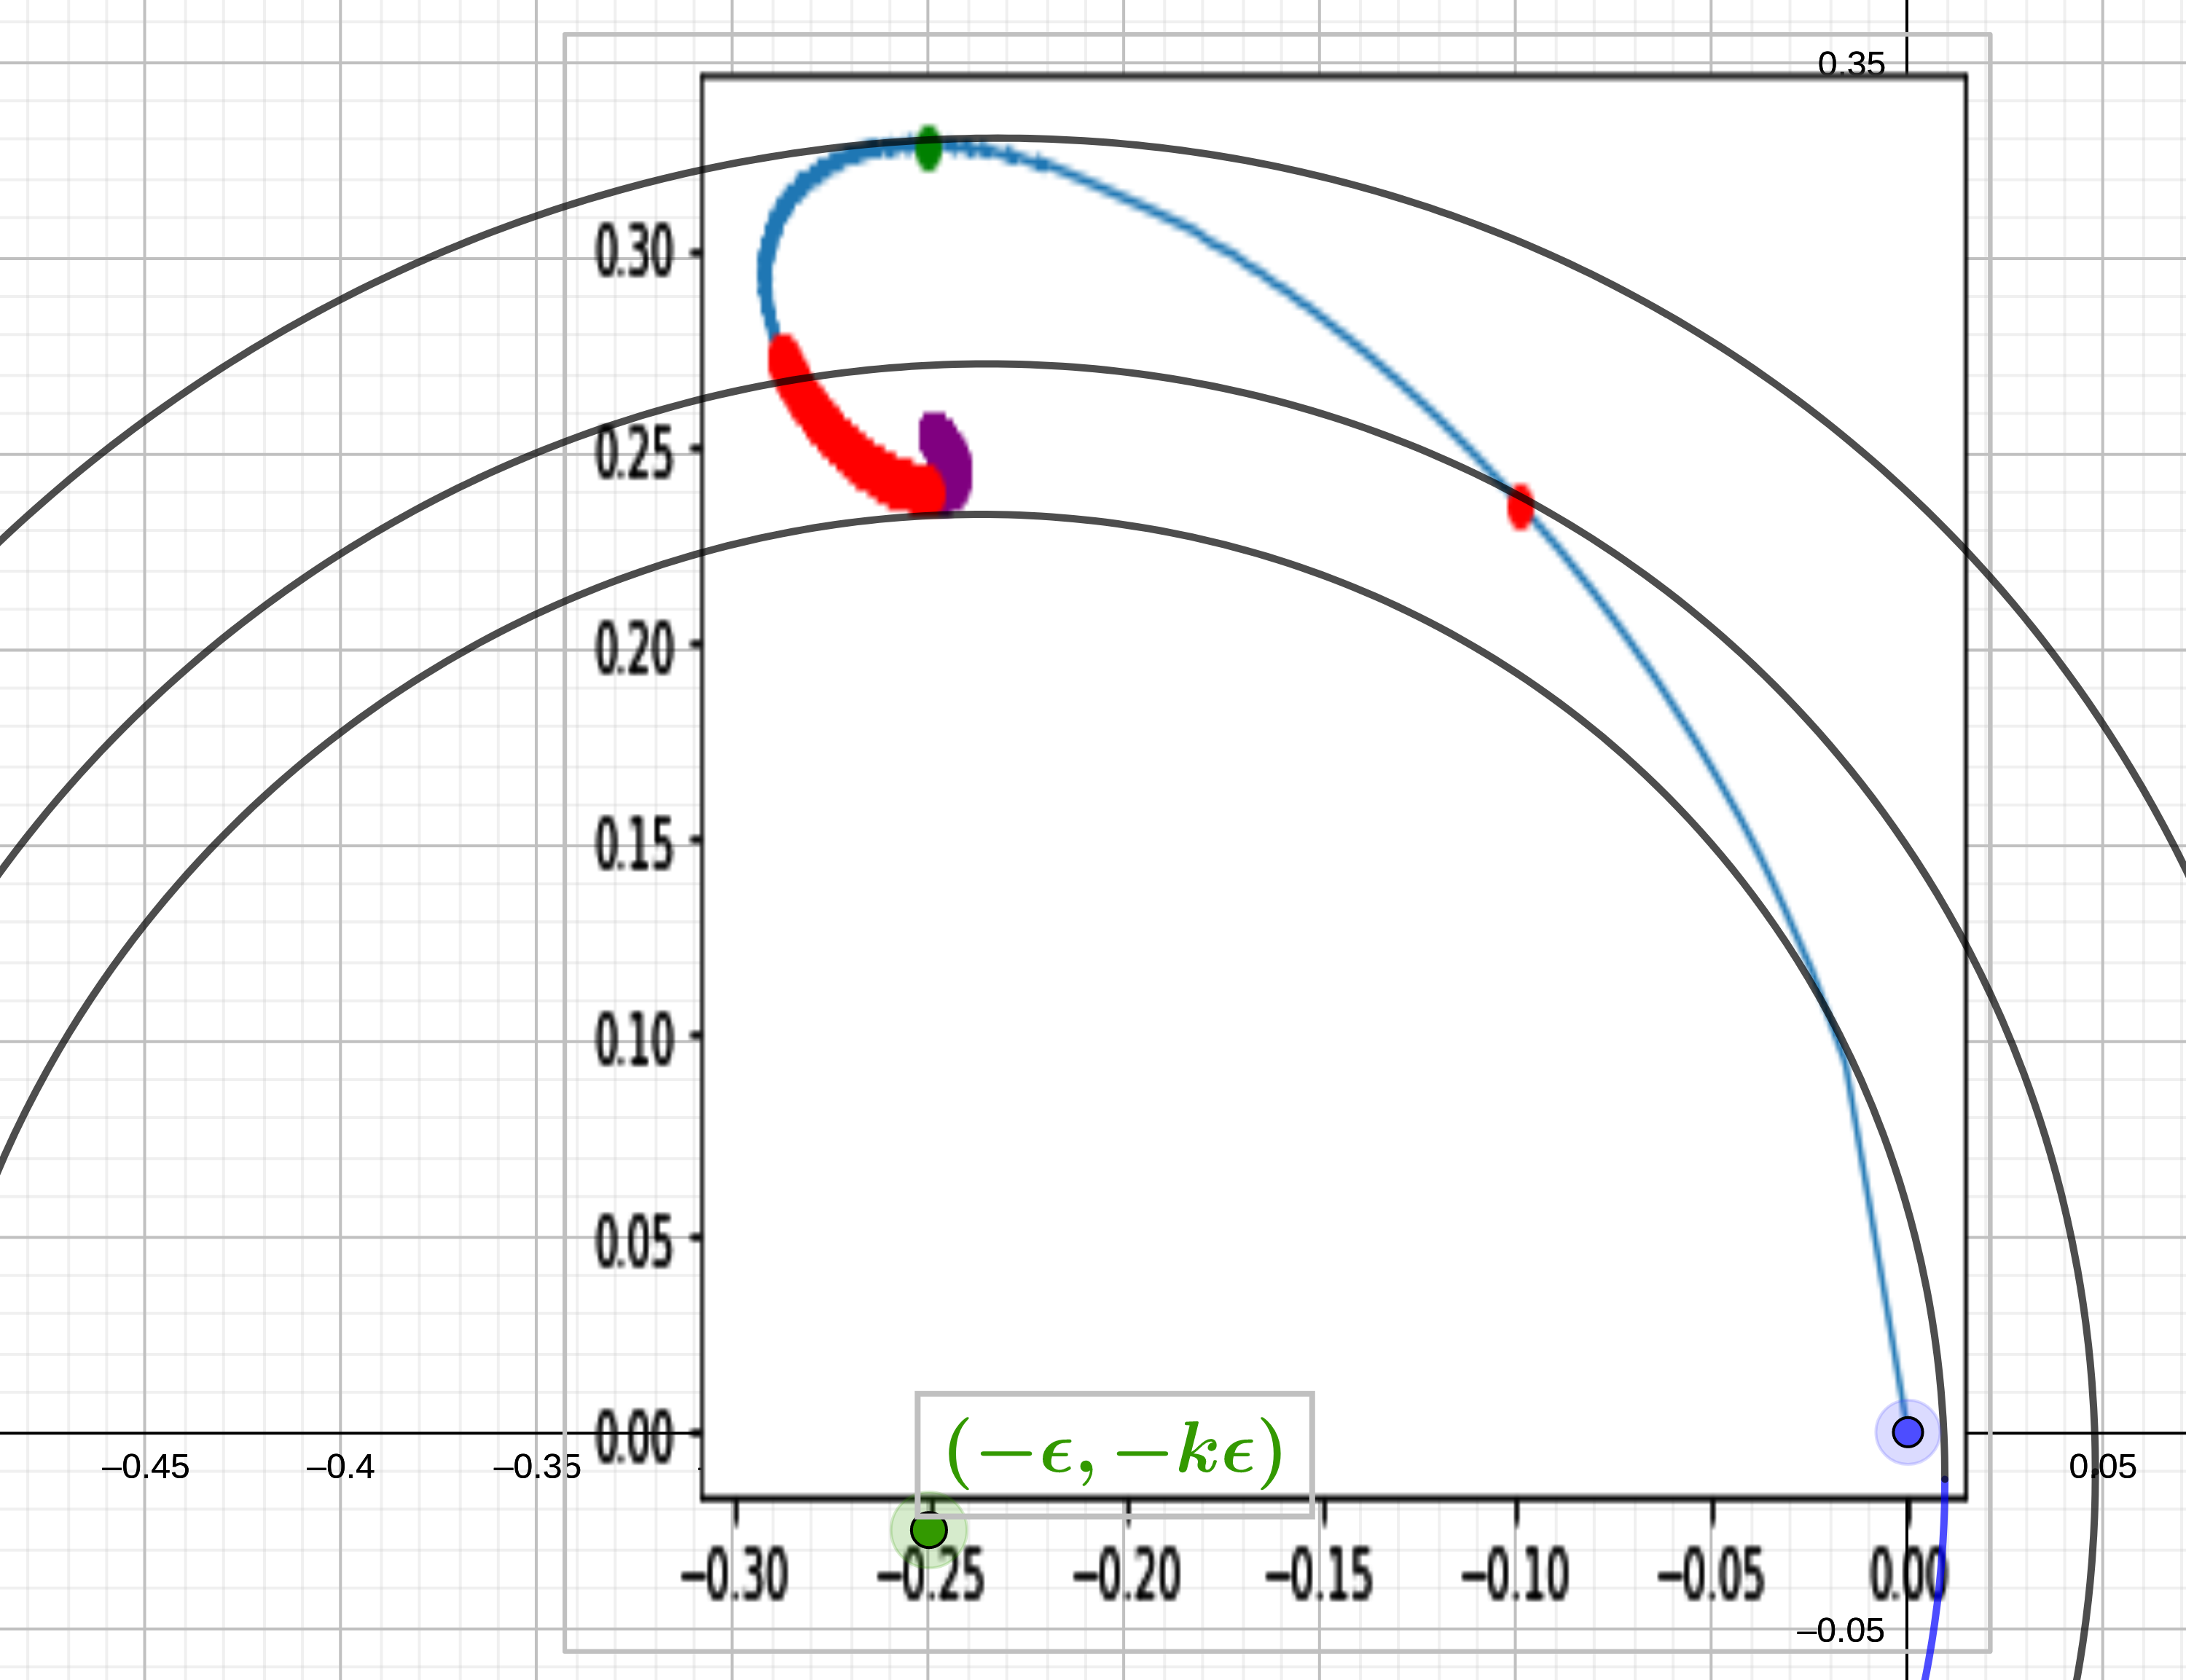
\includegraphics[scale=11]{Elipse_Espiralt.png} \\
\end{tabular}
\end{center}




%%%%%%%%%%%%%%%%%%%%%%%%%%%%%%%%%%%%%%%%%%%%%%%%%%%
\subsection{Analytical expression of the spiral}
Finally, it remains to find the expression of the spiral. Let $(\hat{z},f(\hat{z}),\hat{z})=(\hat{z},-m\hat{z},\hat{z})$ be the initial condition $(x_0,y_0,z_0)$. The expressions of the solutions on the left side are
$$
\begin{array}{l}
x_L(t) = \hat{z} + \epsilon t - \epsilon m + \epsilon e^{-\frac{m}{2}t}
\left(
m \cos (\xi_m t) + \frac{m^2-2}{\sqrt{4-m^2}} \sin (\xi_m t)
\right) \\
y_L(t) = -m(\hat{z}+\epsilon t - \epsilon m) - \epsilon + \epsilon e^{-\frac{m}{2}t}
\left(
(1-m^2) \cos (\xi_m t) + m\frac{3-m^2}{\sqrt{4-m^2}} \sin (\xi_m t)
\right) \\
z_L(t) = \hat{z} + \epsilon t.
\end{array}
$$
We want to find the value of the pair $(y_L,z_L)$ as $x_L(t)=0$. The last equality gives us the expression
\begin{equation}
\hat{z} = - \epsilon t + \epsilon m - \epsilon e^{-\frac{m}{2}t}
\left(
m \cos (\xi_m t) + \frac{m^2-2}{\sqrt{4-m^2}} \sin (\xi_m t)
\right) 
\label{eq:zhat}
\end{equation}
\begin{figure}[h]
    \centering
    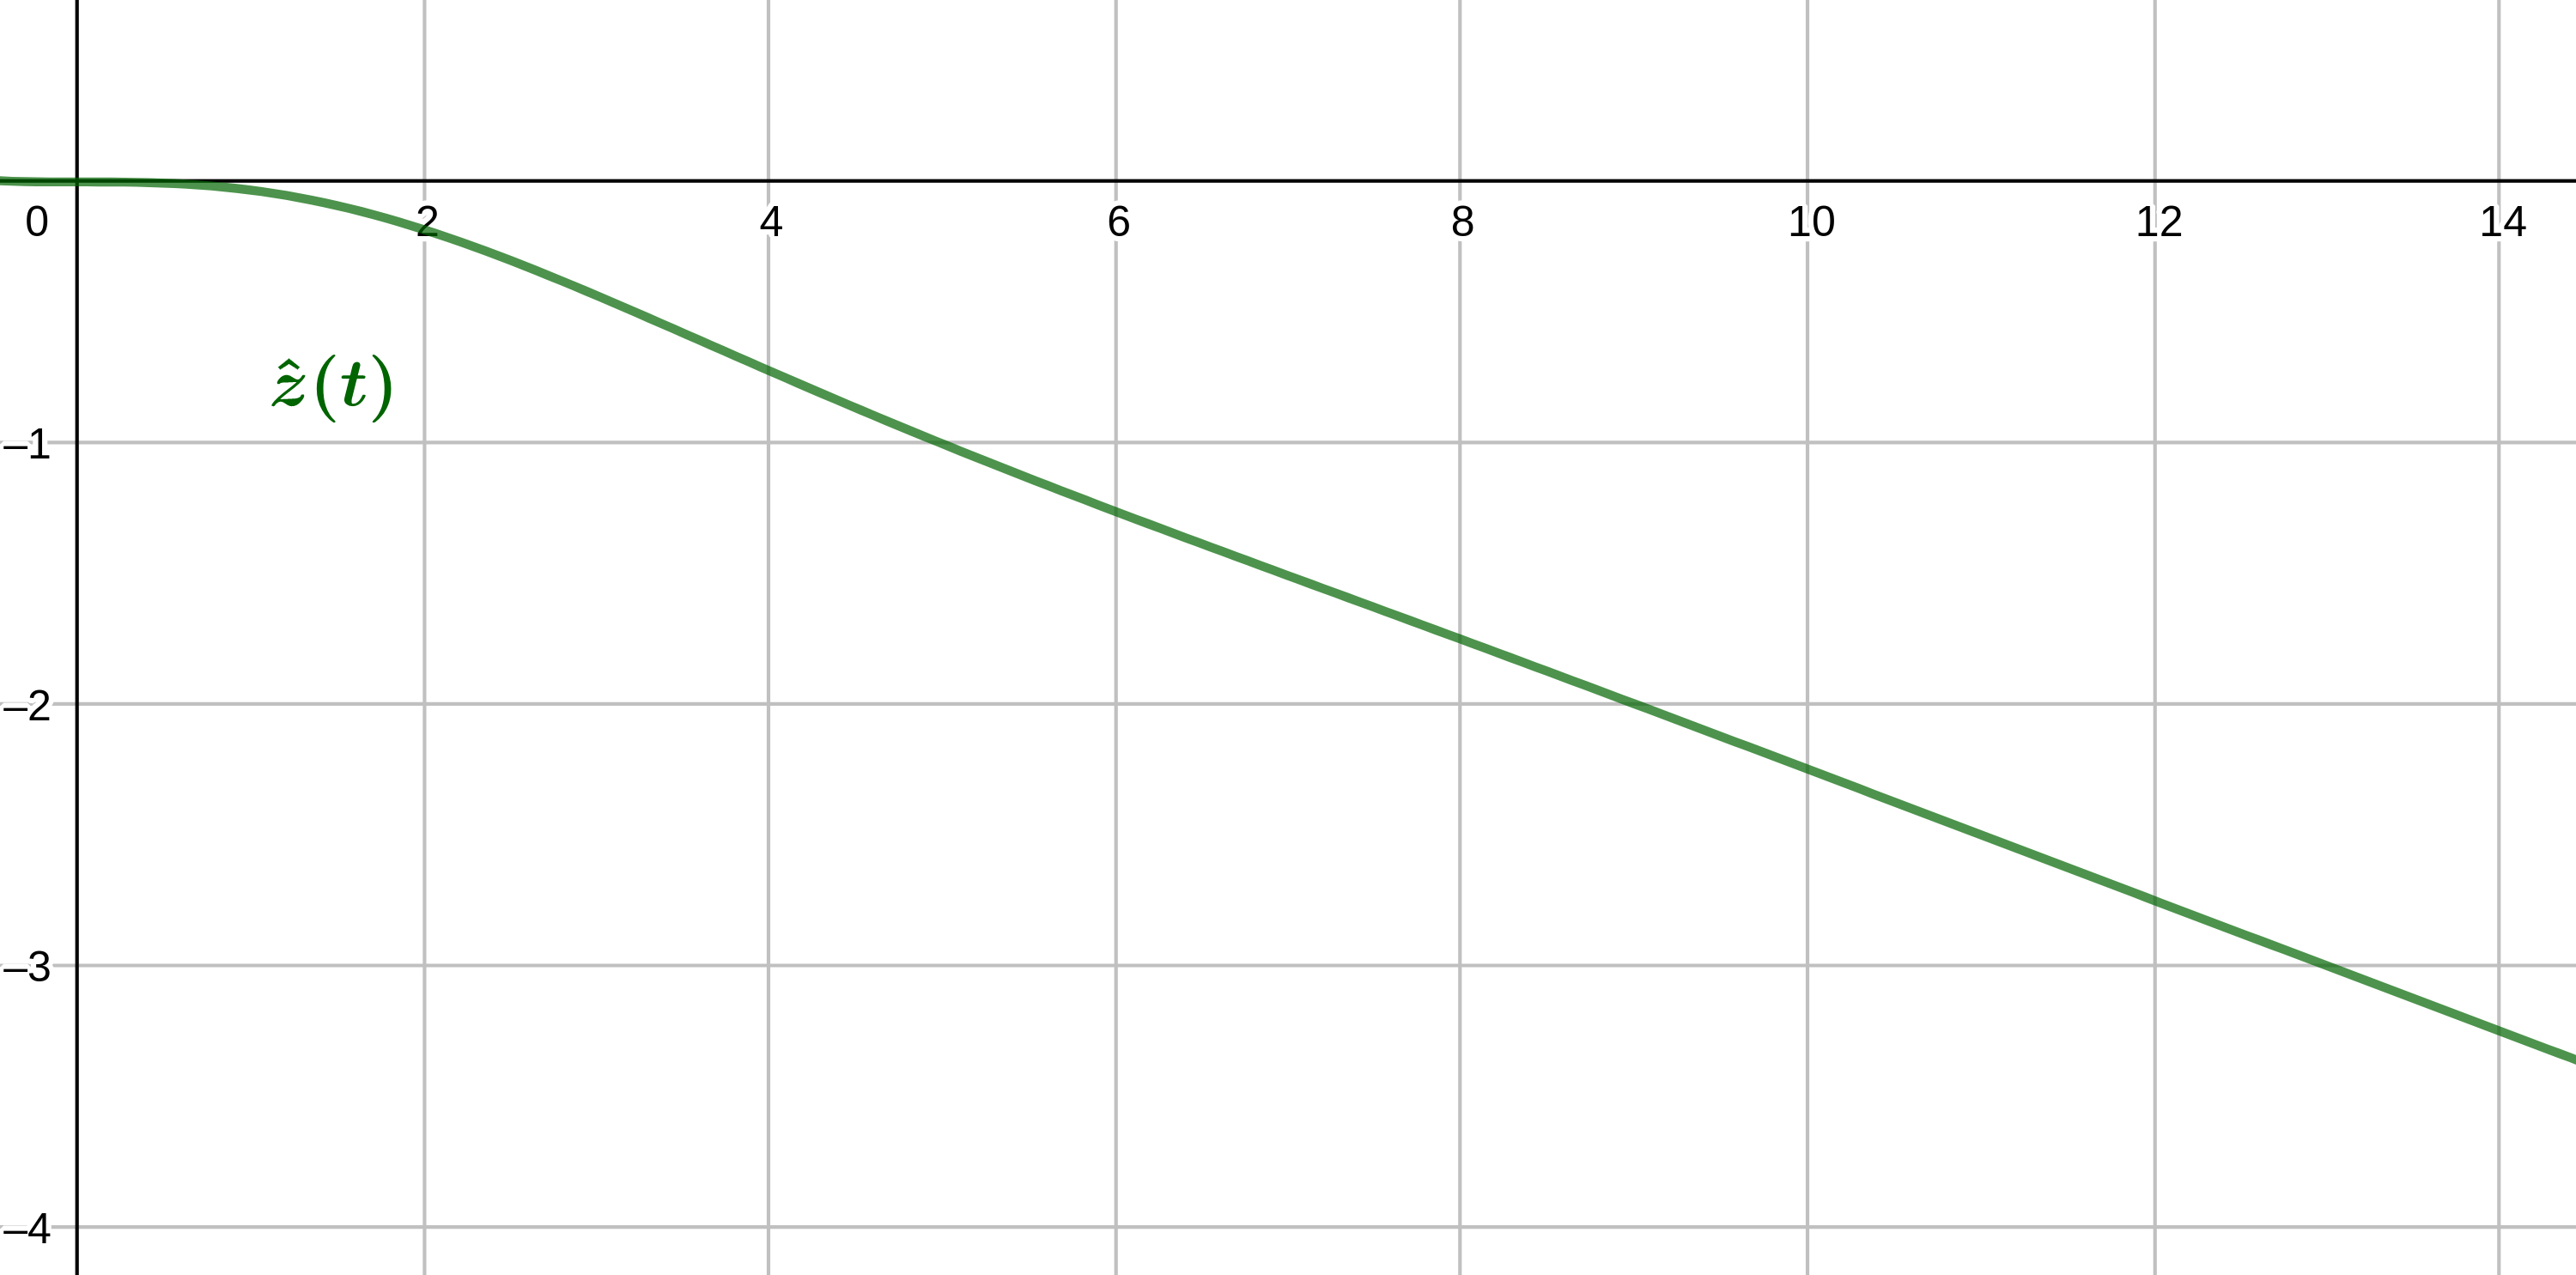
\includegraphics[scale=0.6]{Slow_Passage/hatz_t.png}
    \caption{Plot of $\hat{z}(t)$.}
    \label{fig:hatz}
\end{figure}

In fact, we do not want $\hat{z}$ in terms of $t$, but $t$ in terms of $\hat{z}$. However, it will work as well. Let us give the sketch of the following procedure:
\begin{enumerate}
    \item We will give an injective correspondence between $\hat{z}$ ($\hat{z}<0$) and $t$ ($t>0$).
    \item This will allow us to assure the inverse over all the domain.
    \item Therefore, instead of $(y_L(\hat{z}),z_L(\hat{z}))$, we can use $(y_L(t),z_L(t))$.
\end{enumerate}
We start with Equation \ref{eq:zhat}. We want to assure that it is injective for $t>0$.
$$
\hat{z}'(t) = \epsilon\left[-1+e^{-\frac{m}{2}t}
\left(
\cos(\xi_mt) + \frac{m}{\sqrt{4-m^2}}\sin(\xi_mt)
\right) \right]
$$
We equal the previous expression to $0$, to find the maximum and minimum. That happens if
$$
g(t)=e^{-\frac{m}{2}t}
\left(
\cos(\xi_mt) + \frac{m}{\sqrt{4-m^2}}\sin(\xi_mt)
\right) = 1.
$$
In $t=0$, we have a critical point. However, we will not have another for $t>0$. If we derivate again
$$
g'(t) = -\frac{1}{\xi_m}e^{-\frac{m}{2}t}\sin(\xi_mt)
$$
If we equal to $0$ the last expression, we get that $ t_l = \frac{\pi l}{\xi_m}$ ($l\in\mathbb{N}$) are the times of the critical points. If we substitute in $g$, we have
$$
g(t_l) = (-1)^le^{-\frac{m\pi l}{\sqrt{4-m^2}}}
$$
In absolute value, since $l \geq 0$, we have that $\lvert g(t_l)\rvert <1$ for every $l\neq 0$. All in all, $g(t)$ is less than $1$ for every $t>0$ and thus $\hat{z}(t)$ is a monotone function for $t>0$. Since the function $\hat{z}(t)$ is monotone, we have a bijective correspondence between $\hat{z}\leq 0$ and $t\geq 0$. We can assure the existence of the inverse function $t(\hat{z})$.

As a result, we can use $(y_L(t),z_L(t))$. If we substitute $\hat{z}$ in $y_L$ and $z_L$, we get
$$
\begin{array}{l}
y_L(t) = -\epsilon + \epsilon e^{-\frac{m}{2}t}
\left[
\cos(\xi_m t) + \frac{m}{\sqrt{4-m^2}}\sin(\xi_m t)
\right] \\
z_L(t) = \epsilon m - \epsilon e^{-\frac{m}{2}t}
\left[
m\cos(\xi_m t) + \frac{m^2-2}{\sqrt{4-m^2}}\sin(\xi_m t)
\right]. \\
\end{array}
$$
These expressions are the spirals that we have been plotting computationally.

\begin{figure}[h]
    \centering
    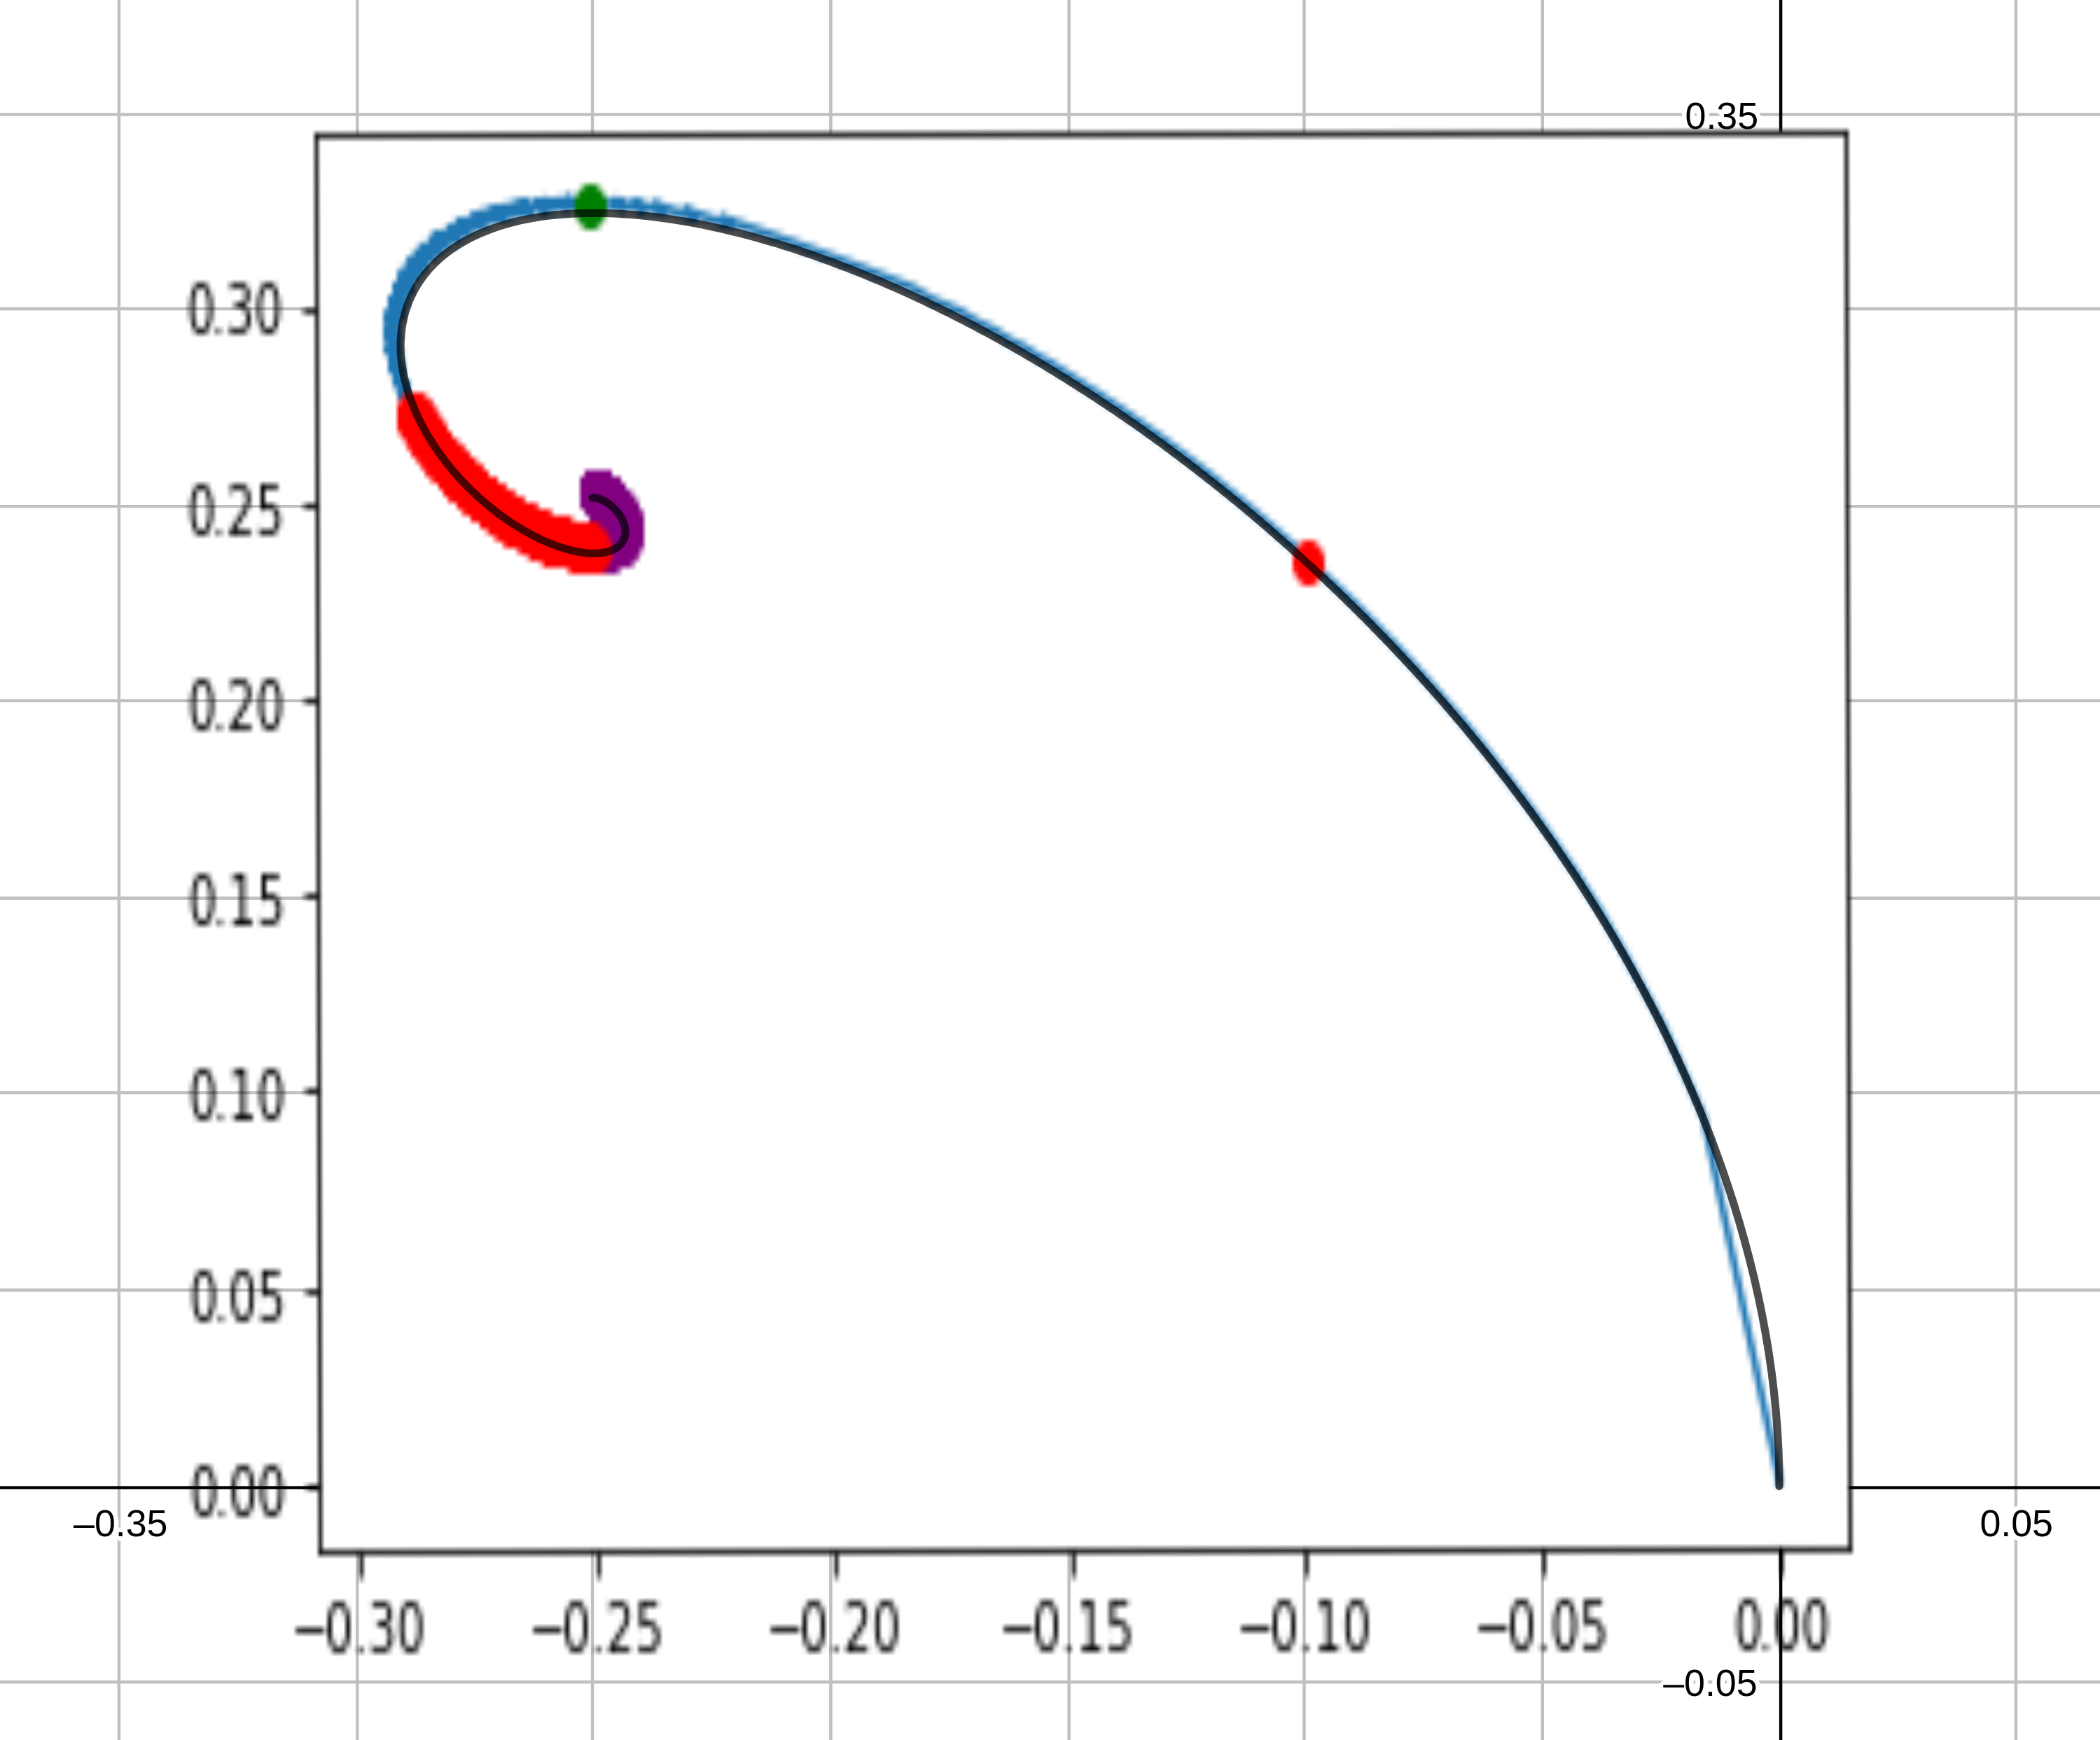
\includegraphics[scale=14]{Slow_Passage/SpiralFitting.png}
    \caption{The black curve is the analytical solution. We can see that the analytical spiral fits well the computational.}
    \label{fig:spiralFitting}
\end{figure}


\break














\subsection{Geometrical approach}
 
Consider the 3D version of the problem given by 
\[
\dot{\mathbf{u}}=
  \left\{
	\begin{array}{ll}
	  A_{-}\mathbf{u}+\mathbf{b} & \text{if } u_1 \leq 0 \\
	  A_{+}\mathbf{u}+\mathbf{b} & \text{if } u_1 \geq 0 
	\end{array}
  \right.,
\]
where
\[
 A_-=\begin{pmatrix}
      -m & -1 & 0 \\
      1 & 0 & -1\\
      0 & 0 & 0
     \end{pmatrix},\quad
 A_+=\begin{pmatrix}
      k & -1 & 0 \\
      1 & 0 & -1\\
      0 & 0 & 0
     \end{pmatrix},\quad
 \mathbf{b}=\begin{pmatrix}
      0 \\
      0 \\
      \varepsilon 
     \end{pmatrix},     
\]

For $\varepsilon =0$, it is known that the system exhibits two invariant sets. One of these invariant sets is given by a poligonal line 
\[
 \left\{
    \begin{array}{ll}
      (x,-mx,x) & \text{if }x\leq 0\\
      (x,kx,x)  & \text{if }x\geq 0      
    \end{array}
 \right.
\]
which is the critical manifold $\mathcal{S}_0$ of the problem and has two branches one attracting (for $x\leq 0$) and one repelling (for $x\geq 0$). The other invariant set is a stable cone foliated by periodic orbits, see Figure \ref{fig:invsets}(a).

\begin{figure}[ht]
 \begin{center}
    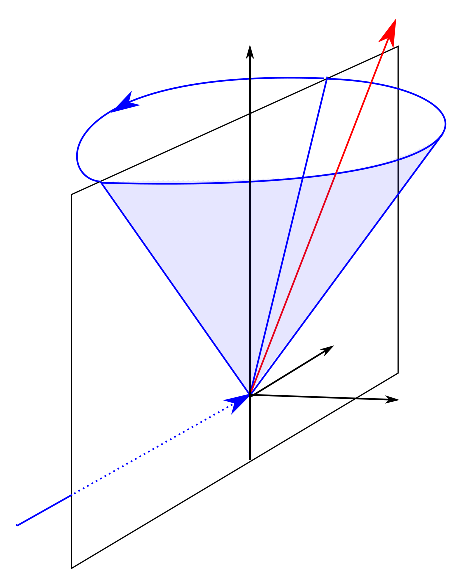
\includegraphics[width=3.7cm]{Sp_PWL_Invset_eps0.eps}\;\;  
    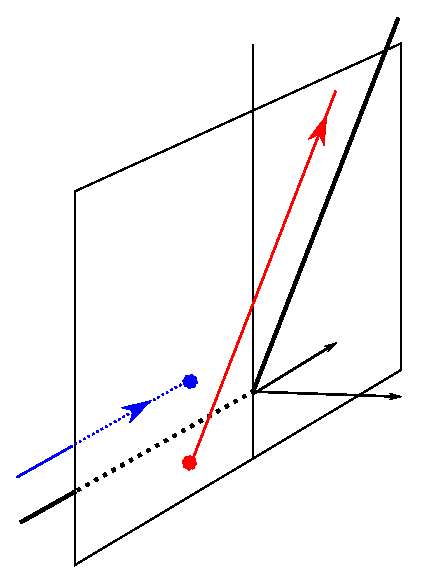
\includegraphics[width=3.7cm]{Sp_PWL_Invset_epsg0.eps}\quad\quad\;
    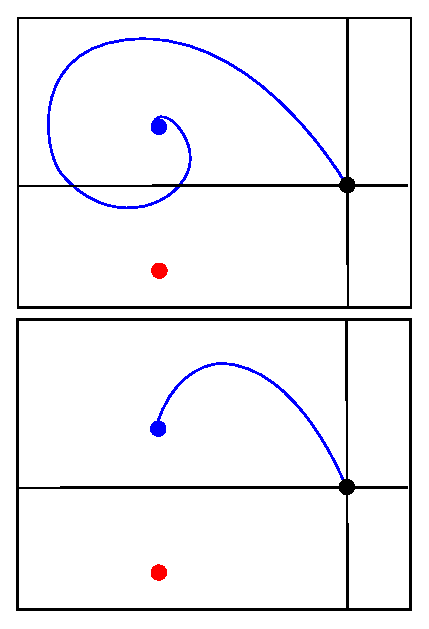
\includegraphics[width=3.7cm]{Sp_PWL_x0_epsg0.eps}  
    \begin{picture}(0,0)
      \put(-310,0){(a)}
      \put(-185,0){(b)}
      \put(-135,150){(c.1)}
      \put(-135,10){(c.2)}
    \end{picture}
 \end{center}
 \caption{\textbf{Invariant objects before and after perturbation:} (a) Slow flow defined over the critical manifold and stable invariant manifold under the fast flow. (b) Attracting and repelling branches of the slow manifold appearing after perturbation of the critical manifold and their intersection points, $\mathbf{p}_{-}=(0,-\varepsilon,m\varepsilon)$ (blue point)  and $\mathbf{p}_{+}=(0,-\varepsilon,-k\varepsilon)$ (red point), with the switching plane $\{x=0\}$ . (c) Image on the switching plane of the attracting branch of the critical manifold by the flow in the half-space $x<0$, (c.1) under focus conditions, (c.2) under node conditions} \label{fig:invsets}
\end{figure}

After perturbation $\varepsilon>0$ see Figure \ref{fig:invsets}(b), the critical manifold perturbs in a slow manifold $\mathcal{S}_{\varepsilon}$ formed by two segments which are the attracting branch $\mathcal{S}_{\varepsilon}^a$ and the repelling branch $\mathcal{S}_{\varepsilon}^r$ given by the solutions 
\begin{align*}
 u_{-}(t)&=\begin{pmatrix} 0 \\ -\varepsilon \\ m\varepsilon \end{pmatrix} +
 \varepsilon t \begin{pmatrix} 1 \\ -m \\ 1 \end{pmatrix},\quad t\leq 0 \\
 u_{+}(t)&=\begin{pmatrix} 0 \\ -\varepsilon \\ -k\varepsilon \end{pmatrix} +
 \varepsilon t \begin{pmatrix} 1 \\ k \\ 1 \end{pmatrix},\quad t \geq 0
\end{align*}
intersecting the plane $\{x=0\}$ are at a distance $O(\varepsilon)$ of the intersection point of critical manifold at the origin.  

\ToDo{Solution $u_+(t)$ should be written in the form given by $x_R$ and $y_R$, and viceversa, solutions $(x_R,y_R)$ should be written as an straight line plus an oscillation. Considering initial conditions at $x=0$ this give us restictions on the initial conditions to remain along a time $\tau$ in a neighbourhood $\delta$ from the $u_+(t)$, which provides a relation between the distance to the slow manifold and the delay.}

\begin{remark}
 The point $\mathbf{p}_-=(0,-\varepsilon,m\varepsilon)$ gives the asymptotic value of the graph of the delay. 
\end{remark}














\section{Study of 3-regions model}

\subsection{Analytic solution}
We take the minimal model
$$
\left\{
\begin{array}{cl}
\dot{x} & = f(x)-y,  \\
\dot{y} & = x-z, \\
\dot{z} & = \epsilon
\end{array}
\right.
$$
with 
$$
f(x) = \left\{
\begin{array}{cc}
-mx & x< -\rho, \\
lx+n & \rho \leq x < \mu \\
kx & x\geq\mu.
\end{array}
\right.
$$
The left and right side of the ODE system is the same as in the previous case. The middle region has a y-intercept non-zero and the solution has a slightly different form.
\begin{align*}
x_C(t) & =a(t) + l\varepsilon +
  e^{\frac{l}{2}t} \left(
      \hat{C}_1 \cos\left(\frac {\sqrt{4-l^2}}2t \right)+
      \hat{C}_2 \sin\left(\frac {\sqrt{4-l^2}}2t \right)
    \right),\\
y_C(t)&=l(a(t)+l\varepsilon)-\varepsilon+n \\
  &+e^{\frac {l}{2}t} \left(
      \frac{l\hat{C}_1-\hat{C}_2\sqrt{4-l^2}}2 \cos\left(\frac {\sqrt{4-l^2}}2t \right)
      +\frac{l\hat{C}_2+\hat{C}_1\sqrt{4-l^2}}2 \sin\left(\frac {\sqrt{4-l^2}}2t \right)
    \right)
\end{align*}


\subsection{First step: centered central region}
We start with the conditions $\rho=-\epsilon\delta$ and $\mu = \epsilon\delta$. This gives us a central region centered, with an amplitude of $2\epsilon\delta$. In this case, to assure continuity, we impose 
$$
l = \frac{k-m}{2}, \quad n = \delta\epsilon\frac{k+m}{2}.
$$
The left-boundary value is
$$
\begin{array}{l}
x(-\delta) = -\epsilon\delta \\
y(-\delta) = -\epsilon+\epsilon\delta m \\
z(-\delta) = m\epsilon-\epsilon\delta .
\end{array}
$$
However, the right-boundary value will change slightly from the theoretical value. Since we want $x( n)=\epsilon\delta$ and $z$ is a decoupled variable, we search the theoretical value of $z$.
$$
z( n)=\epsilon(m+ n) = \epsilon(\delta-k) \rightarrow \boxed{ n = \delta-(k+m)}
$$
In addition, $-\delta<\delta-(k+m)\rightarrow\delta>\frac{k+m}{2}$. Therefore, we have the boundary conditions. Now, we want to find conditions for $\delta$ to connect the manifolds.
$$
\begin{array}{ccccc}
x(-\delta) & = & z(-\delta)+l\epsilon+e^{-l\delta/2}(C_1\cos-C_2\sin) & = & -\epsilon\delta \vspace{0.2cm}\\
y(-\delta) & = & l(z(-\delta)+l\epsilon)-\epsilon+n+ e^{-l\delta/2}((lC_1/2-\xi_lC_2)\cos-(lC_2/2+\xi_lC_1)\sin) & = & -\epsilon+\epsilon\delta m \vspace{0.3cm} \\ %\hline
%y-lx & = & n + e^{-l\delta/2}\left[\left(-\frac{l}{2}C_1-\xi_lC_2\right)\cos -\left(-\frac{l}{2}C_2+\xi_lC_1\right)\sin \right] & = & \epsilon\delta(m+l)
\end{array}
$$
For simplicity, $\sin=\sin(\xi_l\delta)$, $\cos=\cos(\xi_l\delta)$ and $\xi_l=\frac{\sqrt{4-l^2}}{2}$. We want to find $C_1$ and $C_2$. Thus, we can write the equations as
$$
\begin{array}{rrl}
\cos(\xi_l\delta)C_1 & -\sin(\xi_l\delta)C_2 & = -(z(-\delta)+l\epsilon+\epsilon\delta)e^{\frac{l\delta}{2}} \\
\left(\frac{l}{2}\cos(\xi_l\delta)-\xi_l\sin(\xi_l\delta) \right)C_1 & +\left(-\xi_l\cos(\xi_l\delta)-\frac{l}{2}\sin(\xi_l\delta)\right)C_2 & = -(l(z(-\delta)+l\epsilon)+n-\epsilon m\delta)e^{\frac{l\delta}{2}} \\
\end{array}
$$
If we solve the system, the result will be
$$
\begin{pmatrix}
C_1 \\ 
C_2
\end{pmatrix} 
= e^{\frac{l\delta}{2}}\frac{\epsilon(m+l)}{\xi_l}
\begin{pmatrix}
-\xi_l\cos(\xi_l\delta)+\frac{l}{2}\sin(\xi_l\delta) \\
\xi_l\sin(\xi_l\delta)+\frac{l}{2}\cos(\xi_l\delta)
\end{pmatrix}.
$$
Now, we consider the other boundary condition. Let $\lambda=\delta-(k+m)$.
$$
\begin{array}{ccccc}
x(\lambda) & = & z(\lambda)+l\epsilon+e^{l\lambda/2}(C_1\cos+C_2\sin) & = & \epsilon\delta \vspace{0.2cm}\\
y(\lambda) & = & l(z(\lambda)+l\epsilon)-\epsilon+n+ e^{l\lambda/2}((lC_1/2-\xi_lC_2)\cos+(lC_2/2+\xi_lC_1)\sin) & = & -\epsilon+\epsilon\delta k \vspace{0.3cm} \\ %\hline
%y-lx & = & n + e^{l\lambda/2}\left[\left(-\frac{l}{2}C_1-\xi_lC_2\right)\cos %+\left(-\frac{l}{2}C_2+\xi_lC_1\right)\sin \right] & = & \epsilon\delta(k-l)
\end{array}
$$
For simplicity, $\sin=\sin(\xi_l(\delta-(k+m)))$, $\cos=\cos(\xi_l(\delta-(k+m)))$. Now, we finally look for the value of $\delta$. The $x$ equation gives us
$$
\begin{array}{c}
z(\lambda) + l\epsilon + e^{\frac{l\lambda}{2}}\left[C_1\cos + C_2\sin \right] = \epsilon\delta \vspace{0.2cm}\\
\Downarrow \vspace{0.2cm}\\
e^{\frac{l\lambda}{2}}\left[C_1\cos + C_2\sin \right] = \epsilon\delta - (z(\lambda) + l\epsilon ).
\end{array}
$$
The right part of the equality can be simplified as $\epsilon(k-l)=\epsilon\frac{k+m}{2}$. The left side of the equality will transform to
\begin{align*}
e^{l\delta}e^{-\frac{l(k+m)}{2}}\frac{\epsilon(k+m)}{2\xi_l}
& \left(
-(\xi_l\cos(\xi_l(m+k))+\frac{l}{2}\sin(\xi_l(m+k)))\cos(2\xi_l\delta) + \right. \\
&
\left. (\frac{l}{2}\cos(\xi_l(m+k))-\xi_l\sin(\xi_l(m+k)))\sin(2\xi_l\delta)
\right)
\end{align*}
As we simplify in both sides, we get that
$$
\begin{array}{rl}
e^{l\delta} \left(
-(\xi_l\cos(\xi_l(m+k))+\frac{l}{2}\sin(\xi_l(m+k)))\cos(2\xi_l\delta) + \right. 
& = \xi_le^{\frac{l(k+m)}{2}} \\
\left. (\frac{l}{2}\cos(\xi_l(m+k))-\xi_l\sin(\xi_l(m+k)))\sin(2\xi_l\delta)
\right)
\end{array}
$$
Now, we should focus on the 2nd equation. However, it is difficult to manage the expression. We will work with $y-\frac{l}{2}x$, since it will kill the the $lC_i/2$ ($i=1,2$) term in the trigonometric expressions.
$$
\begin{array}{ccc}
y-\frac{l}{2}x & \longrightarrow & e^{l\lambda/2}\left[-\xi_lC_2\cos(\xi_l\lambda) + \xi_lC_1\sin(\xi_l\lambda) \right] = \epsilon l\frac{m+k}{4} \vspace{0.2cm}\\
& \longrightarrow &  \xi_l e^{l\lambda/2}\underbrace{\left[-C_2\cos(\xi_l\lambda) + C_1\sin(\xi_l\lambda) \right]}_{(i)} = \epsilon l\frac{m+k}{4}.
\end{array}
$$
We expand the $(i)$ expression.
$$
\begin{array}{lll}
(i) & = & e^{\frac{l\delta}{2}}\frac{\epsilon(m+k)}{2\xi_l}
\left[
-(\xi_l\cos(\xi_l(m+k))+\frac{l}{2}\sin(\xi_l(m+k)))\sin(2\xi_l\delta) + \right. \vspace{0.2cm}\\
& & \left. (-\frac{l}{2}\cos(\xi_l(m+k))+\xi_l\sin(\xi_l(m+k)))\cos(2\xi_l\delta)
\right]
\end{array}
$$
To sum up, the second equation stands as
$$
\begin{array}{rl}
e^{l\delta}\left[
-(\xi_l\cos(\xi_l(m+k))+\frac{l}{2}\sin(\xi_l(m+k)))\sin(2\xi_l\delta) + \right. 
& = \frac{l}{2}e^{\frac{l(m+k)}{2}}
\\
\left. (-\frac{l}{2}\cos(\xi_l(m+k))+\xi_l\sin(\xi_l(m+k)))\cos(2\xi_l\delta)
\right]
\end{array}
$$
If we put as a linear system, we get ($\sin=\sin(\xi_l(k+m))$, $\cos=\cos(\xi_l(k+m))$)
$$
\begin{array}{c}
\begin{pmatrix}
-\xi_l\cos-\frac{l}{2}\sin & \frac{l}{2}\cos-\xi_l\sin \\ -\frac{l}{2}\cos+\xi_l\sin & -\xi_l\cos-\frac{l}{2}\sin
\end{pmatrix}
\begin{pmatrix}
e^{l\delta}\cos(2\xi_l\delta) \\ e^{l\delta}\sin(2\xi_l\delta) 
\end{pmatrix}
=
e^{l\frac{k+m}{2}}
\begin{pmatrix}
\xi_l \\ \frac{l}{2}
\end{pmatrix} \vspace{0.2cm} \\
\Downarrow \vspace{0.2cm} \\
\begin{pmatrix}
e^{l\delta}\cos(2\xi_l\delta) \\ e^{l\delta}\sin(2\xi_l\delta) 
\end{pmatrix}
=
-e^{l\frac{k+m}{2}}
\begin{pmatrix}
\cos \\ \sin
\end{pmatrix}
\end{array}
$$
All in all, we have
$$
e^{2l\delta} = e^{2l\delta}\cos^2(2\xi_l\delta)+e^{2l\delta}\sin^2(2\xi_l\delta) = e^{l(k+m)} \longrightarrow \boxed{\delta = \frac{k+m}{2}}
$$
However, $\delta$ cannot be this value, since we state that $\delta>\frac{k+m}{2}$.


%%%%%%%%%%%%%%%%%%%%%%%%%%%%%%%%%%%%%%%%%%%%%%%%%%%%%%%%%%%%%%%%%%%%%%%%%%%%%%%%%%%%%%%%%%%%%%%%%%%%%%%%%%%%%%%%%%%%%%%%%%%%%%%%%%%%%%%%%%%%%%%%%%%%%%%%%%%%%%%%%%%%%%%%%%%%%%%%%%%%%%%%%%%%%%%%%%%%%%%%%%%%%%%%%%%%%%%%%%%%%%%%%%%%%%%%%%%%%%%%%%%%%%%%%%%%%%%%%%%%%%%%%%%%%%%%%%%%%%%%%%%%%%%%%%%%%%
\subsection{First step: starting with $t=0$}
We will do the same process, but now we do not start in $t=-\delta$, but in $t=0$. The procedure is similar, and the calculus are simpler. In this case
$$
x(0) = -\epsilon\delta, \quad
y(0) = -\epsilon + \epsilon\delta m, \quad
z(0) = m\epsilon - \epsilon\delta.
$$
The initial conditions $C_1$ and $C_2$ are, respectively,
$$
C_1 = -\epsilon\frac{k+m}{2}, \quad
C_2 = \frac{l}{4\xi_l}\epsilon(k+m)
$$
We want to arrive at $z=-k\epsilon+\epsilon\delta$. This value is given in time $\boxed{\lambda=2\delta-(k+m)}$ The values of $x(\lambda)$ and $y(\lambda)$ must be, respectively,
$$
x(\lambda) = \epsilon\frac{k+m}{2}, \quad
y(\lambda) = l\epsilon\frac{k+m}{2}.
$$
Therefore, if we put it in the boundary of the central region, we have that
$$
\left\{
\begin{array}{lcl}
e^{\frac{l\lambda}{2}}\big(C_1\cos(\xi_l\lambda)+C_2\sin(\xi_l\lambda)\big) & = & \epsilon\frac{k+m}{2} \\
e^{\frac{l\lambda}{2}}\Big((\frac{lC_1}{2}-\xi_lC_2)\cos(\xi_l\lambda) + (\frac{lC_2}{2}+\xi_lC_1)\sin(\xi_l\lambda) \Big) & = & l\epsilon\frac{k+m}{2}.
\end{array}
\right.
$$
We can see it as a linear system in terms of $e^{\frac{l\lambda}{2}}\cos$ and $e^{\frac{l\lambda}{2}}\sin$. If we simplify it, we have
$$
\left\{
\begin{array}{rcrcl}
-2\xi_le^{\frac{l\lambda}{2}}\cos(\xi_l\lambda) & + & le^{\frac{l\lambda}{2}}\sin(\xi_l\lambda) & = & 2\xi_l \\
-2\xi_lle^{\frac{l\lambda}{2}}\cos(\xi_l\lambda) & + & (l^2-2)e^{\frac{l\lambda}{2}}\sin(\xi_l\lambda) & = & 2\xi_ll.
\end{array}
\right.
$$
The solution of the system is
$$
\begin{pmatrix}
e^{\frac{l\lambda}{2}}\cos(\xi_l\lambda) \\ 
e^{\frac{l\lambda}{2}}\sin(\xi_l\lambda)
\end{pmatrix}
=
\frac{1}{4\xi_l}
\begin{pmatrix}
l^2-2 & -l \\
2\xi_ll & -2\xi_l
\end{pmatrix}
\begin{pmatrix}
2\xi_l \\
2\xi_ll
\end{pmatrix}
=
\begin{pmatrix}
 -1 \\ 0
\end{pmatrix}
$$
In this case, it is clear that $e^{\frac{l\lambda}{2}}=1$ and thus either $\lambda=0$ or $l=0$. The first one does not have any sense, since we want a flying time $\lambda>0$. The second time could be possible.









%%%% SECOND STEP
\subsection{Second step: non-centered region}
In the case of a non-centered region, we consider the system where
$$
f(x) = 
\left\{
\begin{array}{cc}
-mx & x<\rho  \\
lx+n & \rho\leq x<\mu \\
kx, & x\geq \mu,
\end{array}
\right. \quad
l = -\frac{m\rho+k\mu}{\rho-\mu}, \quad
n = \rho\mu\frac{k+m}{\rho-\mu}.
$$
\begin{figure}[h]
    \centering
    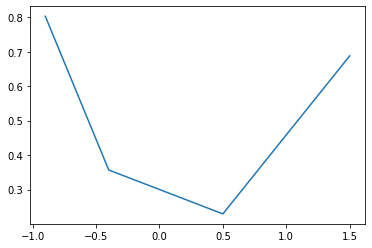
\includegraphics[scale=0.6]{Slow_Passage/f_no_centrat.png}
    \caption{A non-symmetric plot of $f(x)$.}
    \label{fig:f_no_centrat}
\end{figure}

The boundary conditions are
$$
\left\{
\begin{array}{l}
x(0) = \rho  \\
y(0) = -\epsilon - \rho m \\
z(0) = m\epsilon + \rho,
\end{array}
\right. \quad\quad
\left\{
\begin{array}{l}
x(\hat{t}) = \mu \\
y(\hat{t}) = -\epsilon + \mu k \\
z(\hat{t}) = -k\epsilon+\mu,
\end{array}
\right. 
$$
where $\hat{t}=\frac{-\epsilon(k+m)+\mu-\rho}{\epsilon}$. If we want to get the initial condition, we put the boundary conditions to the middle region
$$
\begin{array}{l}
x_C(0) = a_0 + l\epsilon + C_1 = \rho \rightarrow \boxed{C_1 = \frac{\epsilon n}{\rho}} \\
y_C(0) = l(a_0+l\epsilon) - \epsilon -C_2\xi_l+ n+C_1\frac{l}{2} = -\epsilon-\rho m \rightarrow \boxed{C_2 = \frac{-l}{2\xi_l}\frac{\epsilon n}{\rho}}
\end{array}
$$
We write in terms of $ n$ and $l$ because it will be easier to manipulate. Now, we put the other boundary condition.
$$
\begin{array}{l}
x_C(\hat{t}) = -k\epsilon + \mu + l\epsilon + e^{\frac{l}{2}\hat{t}}\big(C_1\cos(\xi_l\hat{t})+\sin(\xi_l\hat{t})\big) = \mu \\
y_C(\hat{t}) = l(-k\epsilon+\mu+l\epsilon) - \epsilon + n + e^{\frac{l}{2}\hat{t}}\big((\frac{l}{2}C_1-\xi_lC_2)\cos(\xi_l\hat{t})  (\frac{l}{2}C_2+\xi_lC_1)\sin(\xi_l\hat{t})\big) = -\epsilon + \mu k
\end{array}
$$
If we simplify, we can write as a linear combination of $e^{\frac{l}{2}\hat{t}}\cos(\xi_l\hat{t})$ and $e^{\frac{l}{2}\hat{t}}\sin(\xi_l\hat{t})$:
$$
\left\{
\begin{array}{rcrl}
e^{\frac{l}{2}\hat{t}}\cos(\xi_l\hat{t}) & + & \frac{-l}{2\xi_l}e^{\frac{l}{2}\hat{t}}\sin(\xi_l\hat{t}) & = \frac{\rho}{\mu} \\
l e^{\frac{l}{2}\hat{t}}\cos(\xi_l\hat{t}) & + & \frac{2-l^2}{\xi_l} e^{\frac{l}{2}\hat{t}}\sin(\xi_l\hat{t}) & = l\frac{\rho}{\mu} \\ 
\end{array}
\right.
$$
The solution of the system is
$$
\begin{pmatrix}
e^{\frac{l}{2}\hat{t}}\cos(\xi_l\hat{t}) \\
e^{\frac{l}{2}\hat{t}}\sin(\xi_l\hat{t})
\end{pmatrix}
=
\frac{1}{2\xi_l}
\begin{pmatrix}
\frac{2-l^2}{\xi_l} & \frac{l}{2\xi_l} \\
-l & 1
\end{pmatrix}
\begin{pmatrix}
\frac{\rho}{\mu} \\ l\frac{\rho}{\mu}
\end{pmatrix}
=
\frac{\rho}{\mu}
\begin{pmatrix}
1 \\ 0
\end{pmatrix}
$$
This gives us $2$ equalities. The 1st one is given by the exponential:
$$
e^{l\hat{t}}=\left(\frac{\rho}{\mu}\right)^2 \rightarrow \boxed{l = \frac{2}{\hat{t}}\ln\left\lvert\frac{\rho}{\mu}\right\rvert}
$$
The second one is given by the trigonometric expressions.
\begin{itemize}
    \item If $\frac{\rho}{\mu}>0$, we have
    $$
    \xi_l\hat{t} = 2\pi p,\ \text{for some }p\in\mathbb{Z}.
    $$
    \item Otherwise, we have
    $$
    \xi_l\hat{t} = \pi + 2\pi p,\ \text{for some }p\in\mathbb{Z}.
    $$
\end{itemize}
\textbf{Note.} If $\rho=-\mu$, we reduce to the previous case, where $l\hat{t}=0$. In this case, we have $l=0$, since the time flying can not be 0.

Let $\xi_l\hat{t} = p\pi$, for $p\in\mathbb{Z}$. From this equality, using the $l$ value of the exponential and $\hat{t}$, we get
\begin{equation} \label{eq:m}
 \boxed{
m = \frac{1}{\epsilon}\left[\mu - \rho - \epsilon k - \epsilon\sqrt{\ln^2\left\lvert\frac{\rho}{\mu}\right\rvert+(p\pi)^2}\right]
}   
\end{equation}
From the exponential equality and the slope value of $n$, we get
\begin{equation} \label{eq:k}
\boxed{
k = \frac{-1}{\mu-\rho}\left(\frac{2\ln\left\lvert\frac{\rho}{\mu}\right\rvert(\rho-\mu)}{\sqrt{\ln^2\left\lvert\frac{\rho}{\mu}\right\rvert+(p\pi)^2}} + \frac{\rho}{\epsilon}\big(\mu-\rho-\epsilon\sqrt{\ln^2\left\lvert\frac{\rho}{\mu}\right\rvert+(p\pi)^2}\big) \right)
}
\end{equation}

\begin{center}
\begin{tabular}{cc}
    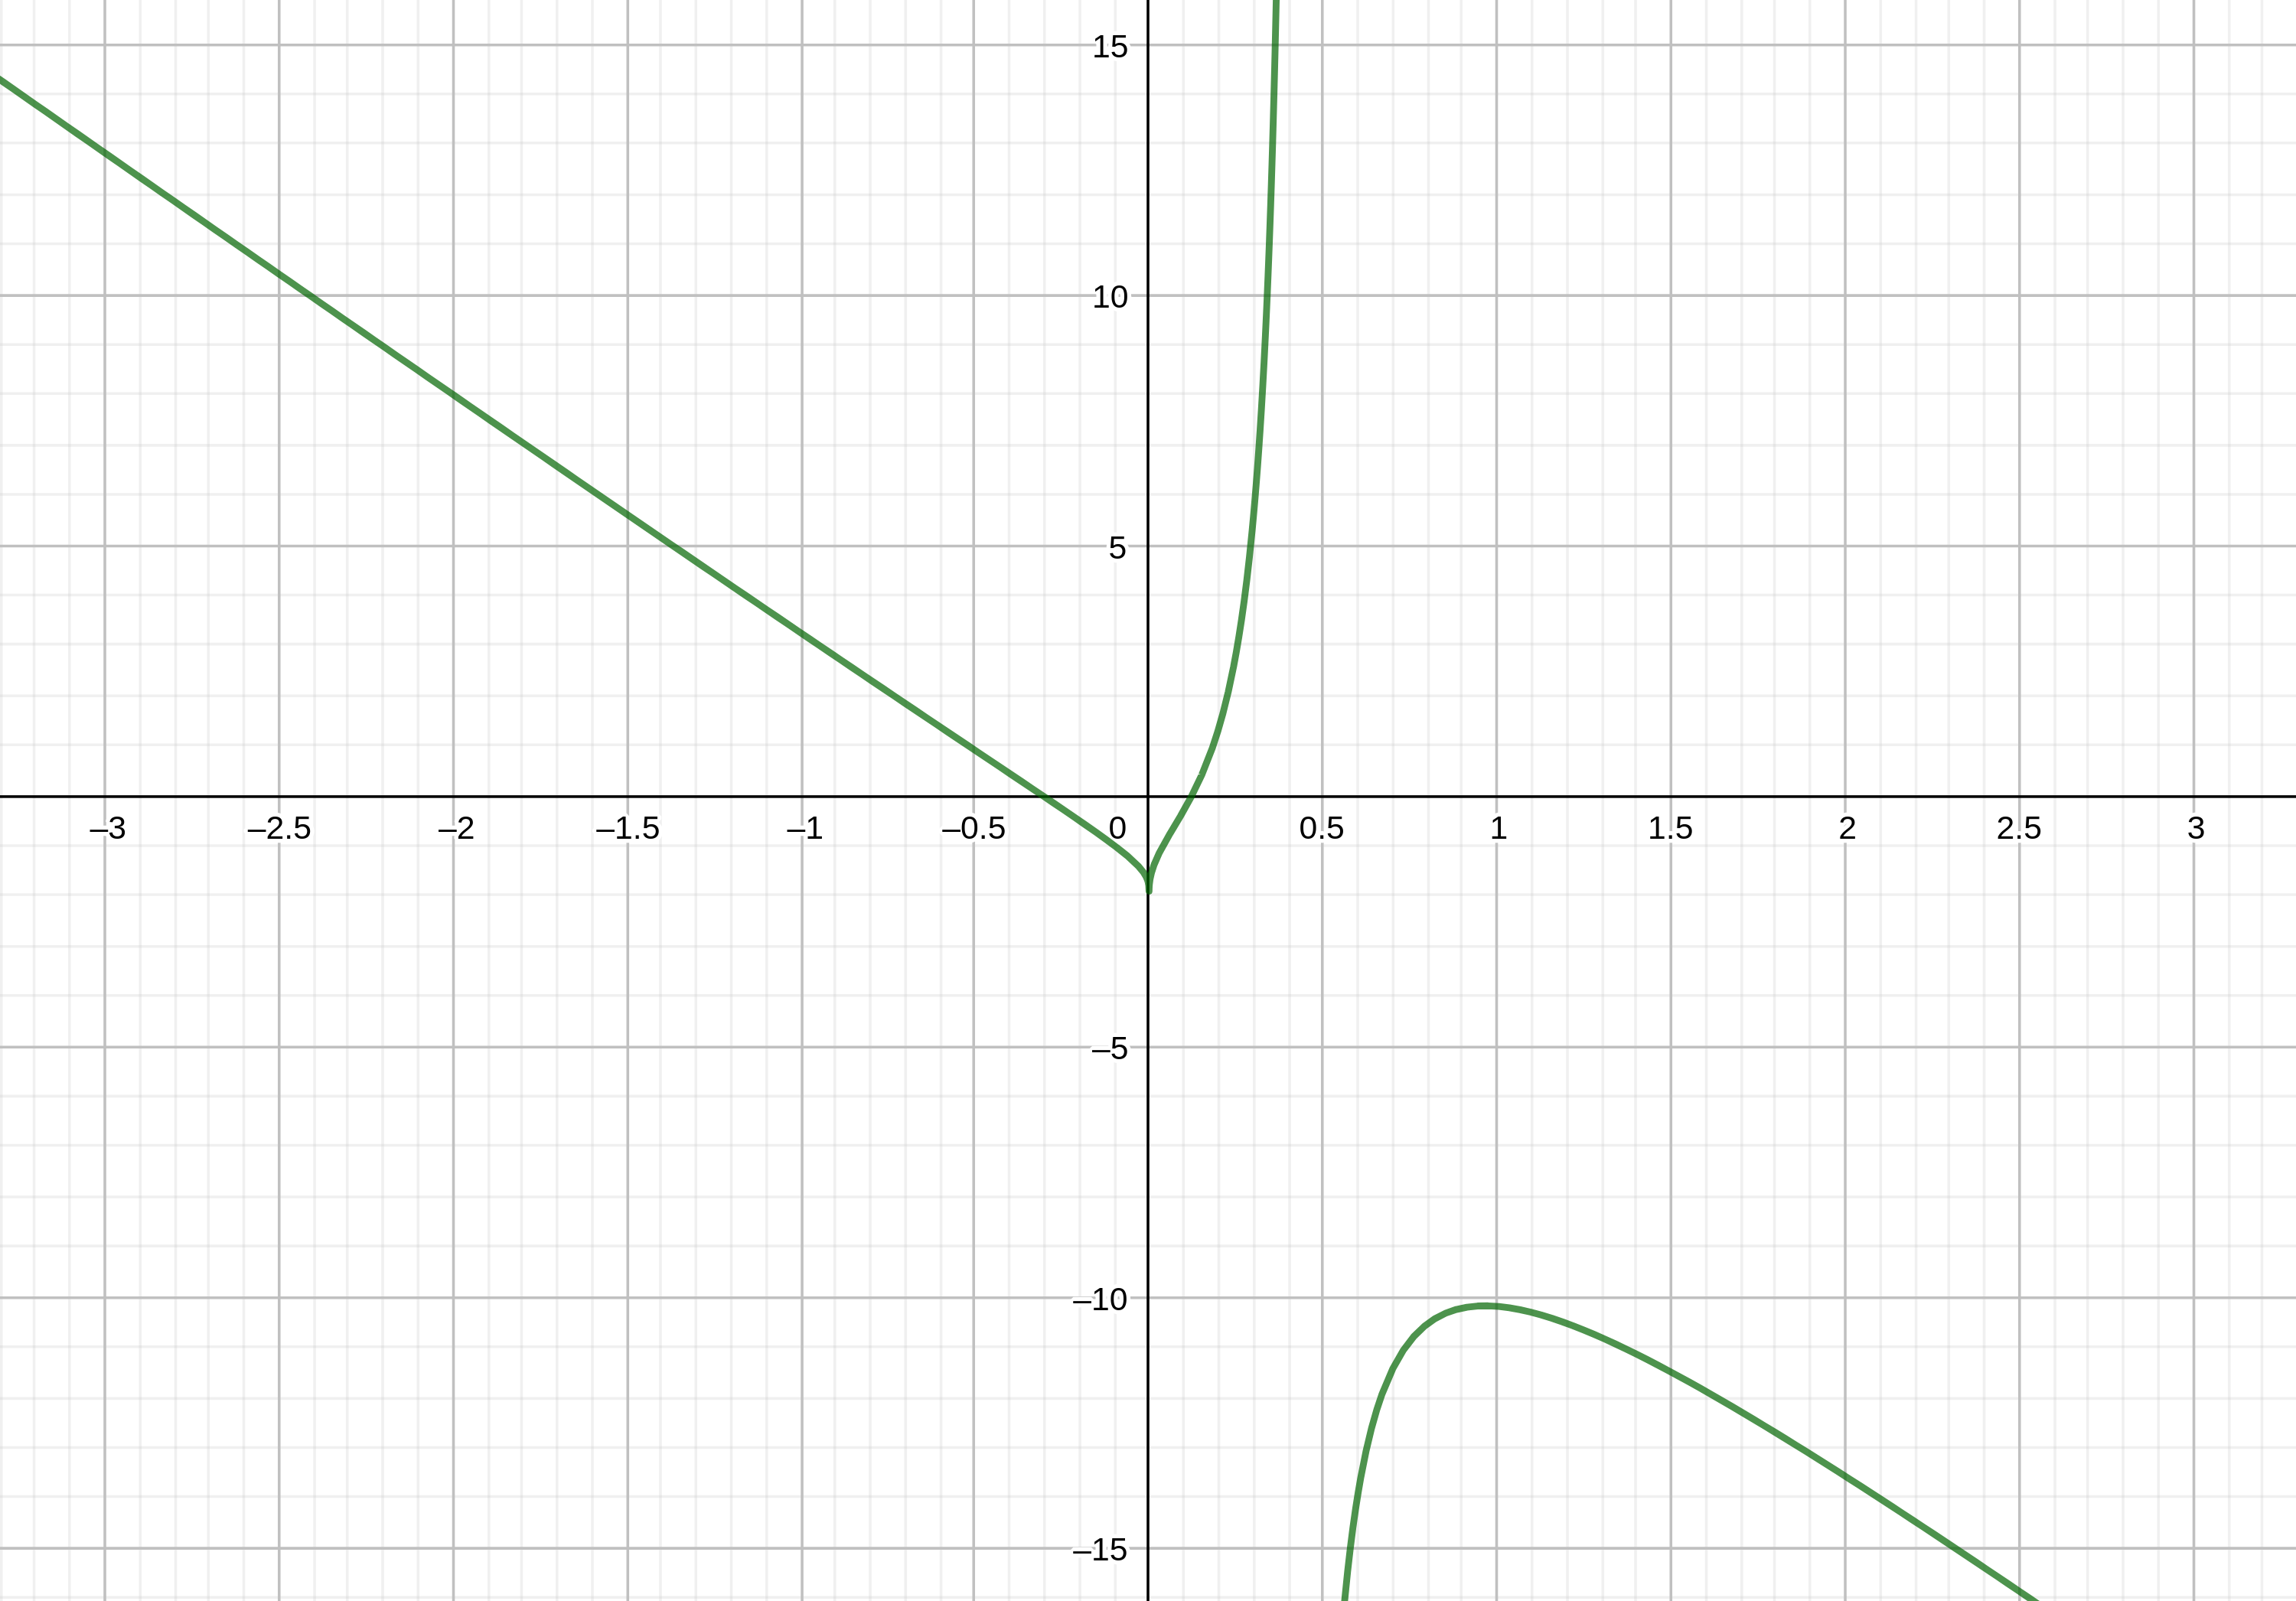
\includegraphics[scale=1]{Slow_Passage/k_rho.png} &
    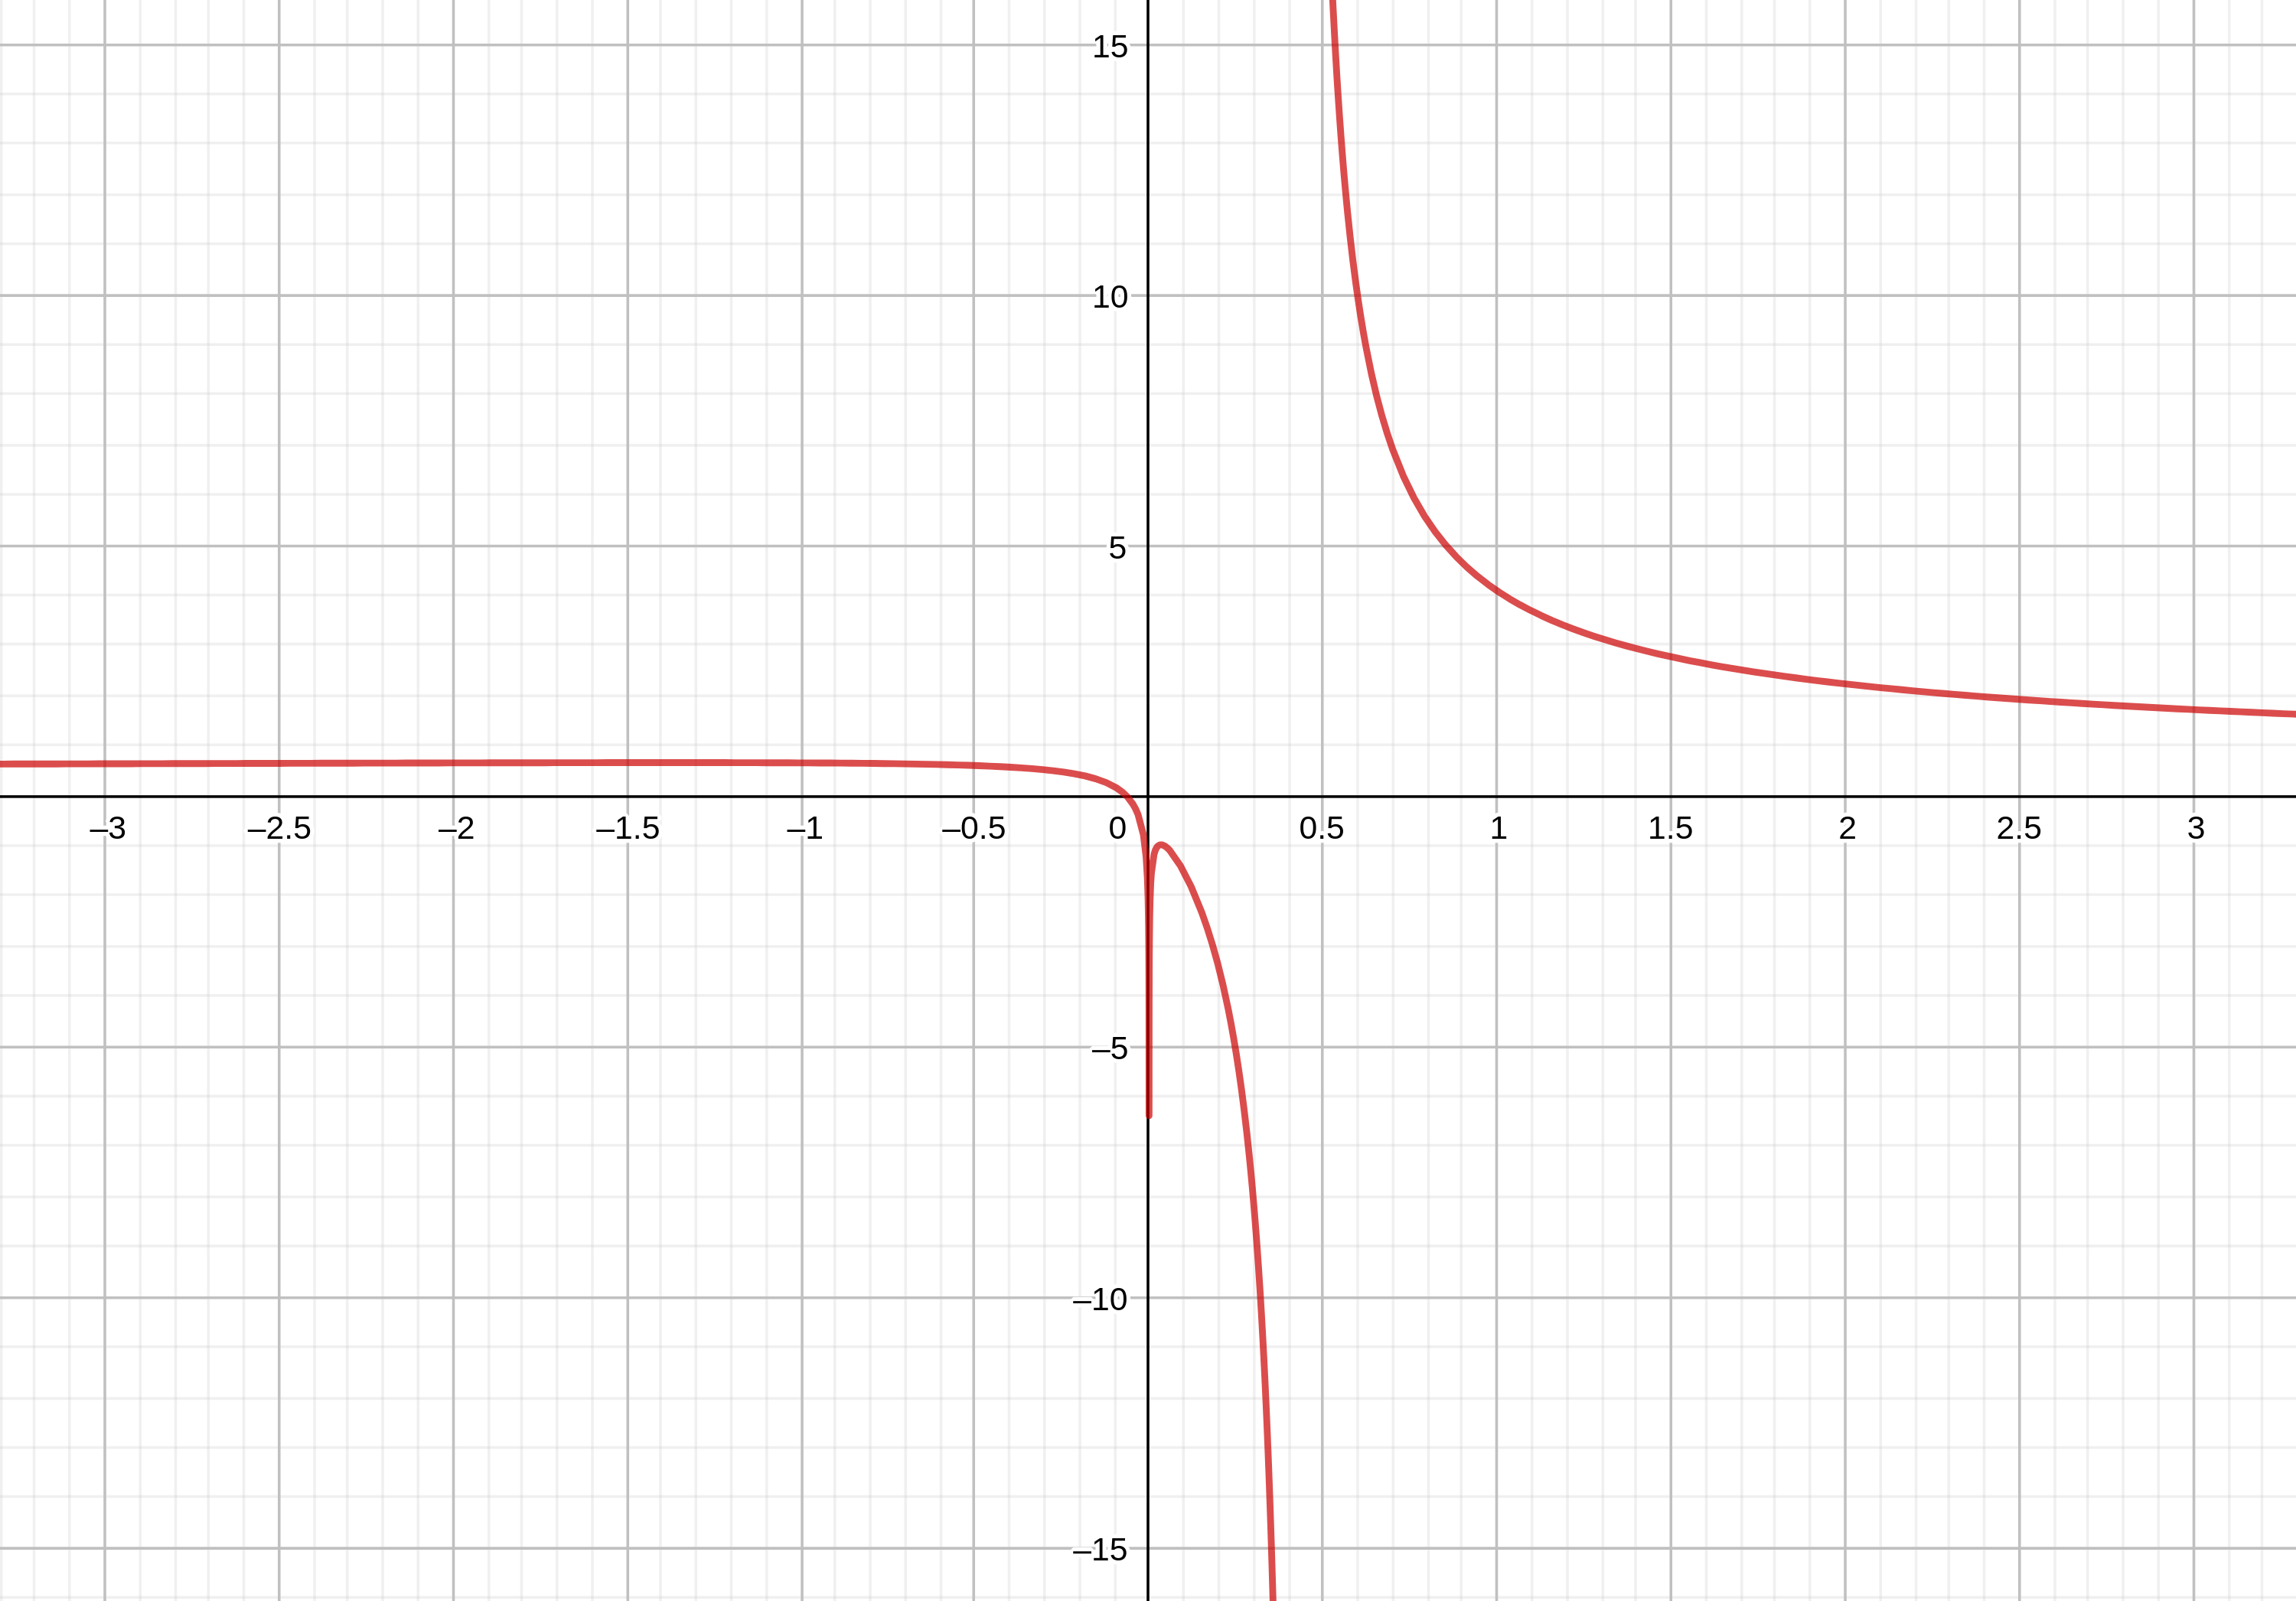
\includegraphics[scale=1]{Slow_Passage/m_rho.png} \\
    $k(\rho)$, for $\epsilon=0.2$, $\mu=0.43$. & $m(\rho)$, for $\epsilon=0.2$, $\mu=0.43$.
\end{tabular}    
\end{center}

Either $p$ is odd or even, it will determine if the sign of $\mu$ and $\rho$ are equal or different. However, it seems that $p$ must be odd. If $p$ is even, it means that we take a lap in the plane $(x,y)$, and at most we want a half lap. Since we want a half lap, we must take $p=1$. %Further, if $p$ is even, it implies that $\mu$ and $\rho$ remains left or right of $x=0$. The absolute value of the slope $l$ is either greater than $m$ or $k$, and we want a slope as plane as possible, since we want to simulate a minimum value.

\subsection{Parameters' selection}
Now, we want to choose $\epsilon$, $\mu$ and $\rho$ such that $0<k<m<2$.\footnote{In fact, we will only use $0<k,m<2$.} Since a general study seems a bit complex, we will realize a local study. Let $m=m(\rho)$ and $k=k(\rho)$. We note that, in case $\rho=-\mu$, equations \ref{eq:m} and \ref{eq:k} gives us
$$
k(-\mu) = m(-\mu) = \frac{\mu}{\epsilon}-\frac{\pi}{2}.
$$
We want to make this expression positive. It happens if $\epsilon<\frac{2\mu}{\pi}$. Moreover, we want this expression to be less than $2$. That is, $\epsilon>\frac{2\mu}{4+\pi}$. Now, we want to study the behavior in a neighborhood of the point $\rho=-\mu$. We calculate the 1st derivate of $m$ and $k$.
$$
\frac{dm}{d\rho} = \frac{2(\ln^2\left\lvert\frac{\mu}{\rho}\right\rvert-\pi^2)}{\rho(\ln^2\left\lvert\frac{\mu}{\rho}\right\rvert+\pi^2)^{\frac{3}{2}}} -
\frac{\mu}{\rho(\mu-\rho)^2\sqrt{\ln^2\left\lvert\frac{\mu}{\rho}\right\rvert+\pi^2}}
\left[
\rho(\ln^2\left\lvert\frac{\mu}{\rho}\right\rvert+\pi^2)-(\mu-\rho)\ln\left\lvert\frac{\mu}{\rho}\right\rvert
\right]
$$
$$
\frac{dk}{d\rho} = -\frac{2(\ln^2\left\lvert\frac{\mu}{\rho}\right\rvert-\pi^2)}{\rho(\ln^2\left\lvert\frac{\mu}{\rho}\right\rvert+\pi^2)^{\frac{3}{2}}} +
\frac{\mu}{(\mu-\rho)^2\sqrt{\ln^2\left\lvert\frac{\mu}{\rho}\right\rvert+\pi^2}}
\left[
(\ln^2\left\lvert\frac{\mu}{\rho}\right\rvert+\pi^2)+\frac{2(\mu-\rho)}{\mu}\ln\left\lvert\frac{\mu}{\rho}\right\rvert
\right] 
- \frac{1}{\epsilon}
$$
If we evaluate in $\rho=-\mu$, we get
$$
\left.
\frac{dm}{d\rho}
\right\rvert_{\rho=-\mu} =
\frac{8-\pi^2}{4\pi\mu}, \quad
\left.
\frac{dk}{d\rho}
\right\rvert_{\rho=-\mu} =
-\frac{8-\pi^2}{4\pi\mu} - \frac{1}{\epsilon}
$$
We want to find a region such that $m>k$. Thus, we evaluate the difference in the derivate of the point
$$
\left.\left(\frac{dm}{d\rho}-\frac{dk}{d\rho}\right)\right\rvert_{\rho=-\mu} 
=
\frac{8-\pi^2}{2\pi\mu} + \frac{1}{\epsilon}
$$
This difference will be positive if $\epsilon<\frac{2\pi\mu}{\pi^2-8}$. However, we can check that $\frac{2\mu}{\pi}<\frac{2\pi\mu}{\pi^2-8}$. Hence, for $\epsilon\in]\frac{2\mu}{4+\pi},\frac{2\mu}{\pi}[$, there is a neighborhood (sign-preserving property) where this difference will increase as $\rho$ increases.

All in all, we have that, given $\mu$, for $\epsilon\in]\frac{2\mu}{4+\pi},\frac{2\mu}{\pi}[$, every $\rho\in]-\mu,-\mu+\hat{\epsilon}[$ gives us a good pair $(m,k)$, for $\hat{\epsilon}>0$ sufficiently small.

\textbf{Notes.} We note that, as $\epsilon\to 0$, $\mu\to 0$. In addition to, since $-\mu<\rho<-\mu+\hat{\epsilon}<0$ (we recall that $\rho<0$) and $\mu\to 0$, it happens that $\rho\to 0$.

\subsection{Simulations}
\textbf{CASE \boldmath$\mu\neq-\rho$:} Now, we plot a simulation with a certain value to show the slow passage phenomena. Let $\epsilon = 0.2$, $\rho = -0.4$ and $\mu = 0.5$. For these values, $\epsilon$ is in the desired interval and we get the values $k\approx 0.45852$, $m\approx 0.89197$, that satisfies $0<k<m<2$.

\begin{figure}[h]
\begin{tabular}{cc}
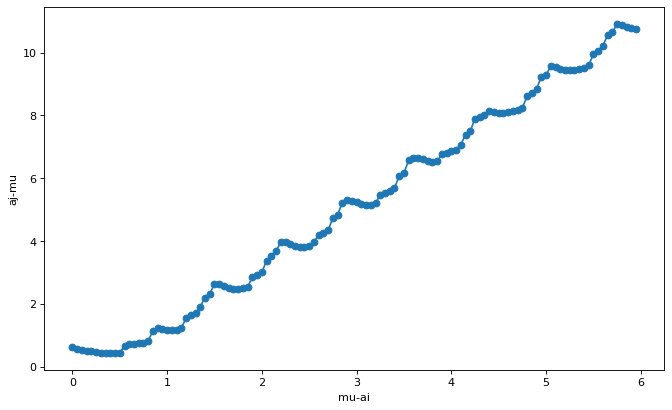
\includegraphics[scale=0.34]{Slow_Passage/SP3Dline.png} &
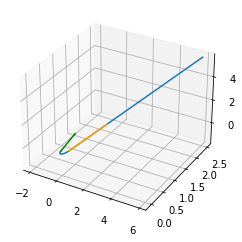
\includegraphics[scale=0.6]{Slow_Passage/SP3Dcurve.png}
\end{tabular}
\caption{On the left, the delay plot as we start over the line $x=a$, $y=f(a)$. We can imagine a straight line fitting the curve. On the right side, we can see the connection between the left side (green) and the right side (orange).}
\label{fig:SP3D}
\end{figure}

The straight line  has also a delay at the beginning, because while we do not pass to the left region, the central region will works as in the 2 region problem. In this case, the plot of $x=\mu$ is not exactly an spiral, even though it tends to the real equilibrium point.

\begin{figure}[h]
    \centering
    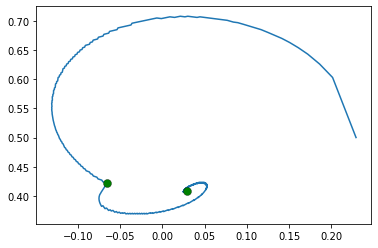
\includegraphics[scale=0.6]{Slow_Passage/NewSpiral.png}
    \caption{Images from $(a,f(a),a)$ at the plane $x=\mu$. The 1st green point starts at $a=\rho$. The 2nd is the point $(-\epsilon+\mu k, -k\epsilon+\mu$). This point is the limit of the plot.}
    \label{fig:new.spiral}
\end{figure}



\textbf{CASE \boldmath$\mu=-\rho$:} Now, we plot a simulation with a certain value to show the slow passage phenomena. The equal case is special, since it implies $k=m$ and $l=0$. The field is symmetric and it reminds a parabola. 

Let $\epsilon = 0.05$, $\rho = -0.15$ and $\mu = 0.15$. For these values, $\epsilon$ is in the desired interval and we get the values $k=m=\approx 1.42920$.

\begin{figure}[h]
\begin{tabular}{cc}
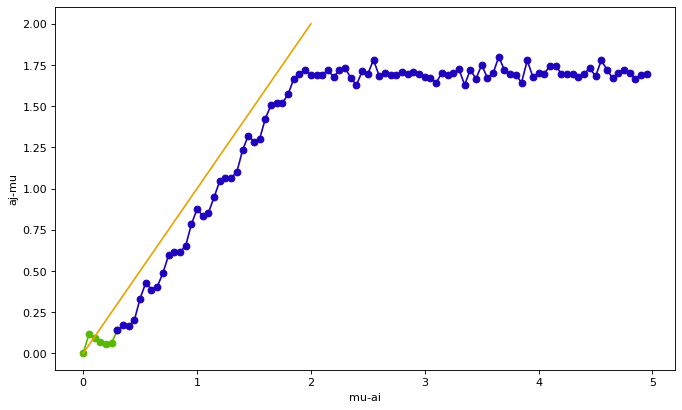
\includegraphics[scale=0.34]{Slow_Passage/SPplot_keqm.png} &
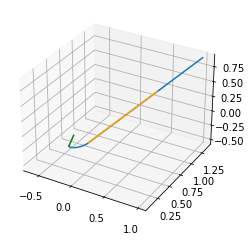
\includegraphics[scale=0.6]{Slow_Passage/SP3Dline_keqm.png}
\end{tabular}
\caption{On the left, the delay plot as we start over the line $x=a$, $y=f(a)$. The identity fits the curve until $\mu-a_i=2$, but with a little displacement. Moreover, we can see the delay at the beginning (green) and a collapse in $\mu-a_i=2$. On the right side, we can see the connection between the left side (green) and the right side (orange).}
\label{fig:SP3D.keqm}
\end{figure}

Finally, we plot the spiral

\begin{figure}[h]
    \centering
    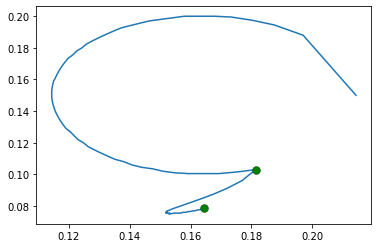
\includegraphics[scale=0.6]{Slow_Passage/Spiral_keqm.png}
    \caption{Images from $(a,f(a),a)$ at the plane $x=\mu$. The 1st green point starts at $a=\rho$. The 2nd is the point $(-\epsilon+\mu k, -k\epsilon+\mu$).}
    \label{fig:spiral.keqm}
\end{figure}





%%%%%%%%%%%%%%%%%%%% Ellipse in 3-linear region
\subsection{Ellipses in 3 linear regions}
Let $x(t)=\rho$. We want to find the analytical expression of the ellipses that escpes with the same time.
$$
\begin{array}{l}
x_C(0) = a_0+l\epsilon + C_1 = \rho \longrightarrow \boxed{C_1 = \rho-a_0-l\epsilon} \\
y_C(0) = l(a_0+l\epsilon)-\epsilon+n+D_1 = y_0 \longrightarrow \boxed{D_1 = (y_0+\epsilon-n)-l(a_0+l\epsilon)} \\
C_2 = \frac{1}{\xi_l}(\frac{l}{2}C_1-D_1) \longrightarrow \boxed{C_2 = \frac{1}{\xi_l}(\frac{l}{2}(\rho+a_0+l\epsilon)-(y_0+\epsilon-n))} \\
D_2 = \frac{l}{2}C_2 + \xi_lc_1 \longrightarrow \boxed{D_2 = \frac{1}{\xi_l}(-\frac{l}{2}(y_0+\epsilon-n)+(\rho-(a_0+l\epsilon))+\frac{l^2}{2}(a_0+l\epsilon))}
\end{array}
$$
Now, we can write $z_C(t)$ in terms of $x_C(t)$ as
$$
z_C(t) = x_C(t)-l\epsilon - e^{\frac{l}{2}t}(C_1\cos(\xi_lt)+C_2\sin(\xi_lt))
$$
We compute $C_1^2+C_2^2$:
$$
\begin{array}{c}
(\rho-(a_0+l\epsilon))^2 + \frac{1}{\xi_l^2}(\frac{l}{2}(\rho +(a_0+l\epsilon))-(y_0+\epsilon-n))^2 = d \\
\Downarrow \\
\frac{1}{\xi_l^2}[(a_0+l\epsilon-\rho)^2 + (y_0+\epsilon-n)^2-l(y_0+\epsilon-n)(\rho+a_0+l\epsilon)] = d
\end{array}
$$
We study the particular case where $m=k$. Thus,
$$
(a_0-\rho)^2 +(y_0+\epsilon+\rho)^2 = d.
$$
We can put $y_0$ in terms of $a_0$ as $y_0 = -(\epsilon+\rho)\pm\sqrt{d-(a_0-\rho)^2}$. Now, we want to translate these ellipses to the plane $x=\mu$. This must verify
$$
\begin{array}{l}
y_C(t) = -\epsilon +n \pm \sqrt{d-(a_0-\rho)^2}\cos(t) + (\rho-a_0)\sin(t) \\
z_C(t) = \mu -(\rho-a_0)\cos(t)\pm\sqrt{d-(a_0-\rho)^2}\sin(t).
\end{array}
$$
As we know, $a\cos x+b\sin x=c\cos(x+\varphi)$, where $c=sgn(a)\sqrt{a^2+b^2}$ and $\varphi=\arctan(-\frac{b}{a})$. Therefore, since $c^2=d$, the point $(a_0,y_0(a_0))$ on the ellipse does not depend on. Fixed $a_0$, we can get the image moving $t$.

\begin{figure}[h]
    \centering
    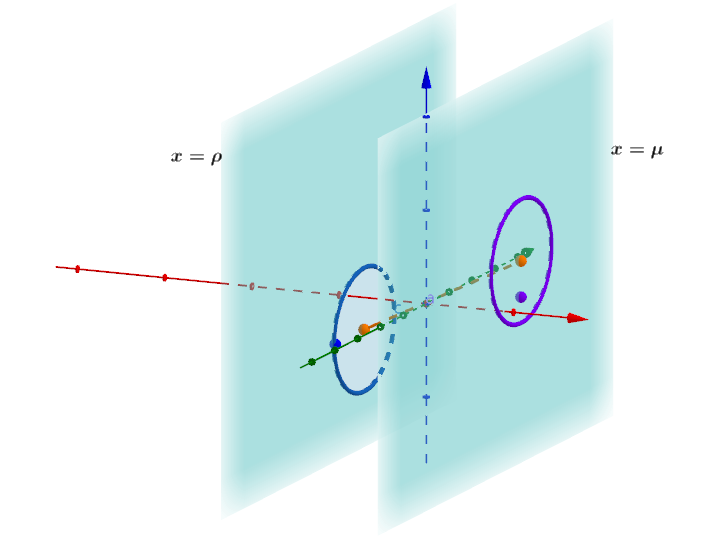
\includegraphics[scale=0.4]{Slow_Passage/3dEllipse_transformation.png}
    \caption{Ellipse transformation from plane $x=\rho$ to $x=\mu$.}
    \label{fig:ell.trans}
\end{figure}







\end{document}